% RASCUNHO. Resultados das fases 11 a 13, no formato de ic_report.tex.
% Compilar a partir de report/:  latexmk -pdf artigo_kernel.tex
% As figuras vêm direto de results/figures_generated/. \pendente{...} marca, em vermelho, o que depende
% das seeds 43 e 44 da fase 13 (jobs 835245, 835347 e 835352).
\documentclass[conference]{IEEEtran}
\IEEEoverridecommandlockouts
\renewcommand{\figurename}{Figura}
\renewcommand{\tablename}{Tabela}
\renewcommand{\appendixname}{Apêndice}
\renewcommand{\abstractname}{Resumo}
\usepackage{cite}
\usepackage{amsmath,amssymb,amsfonts}
\usepackage{graphicx}
\usepackage{textcomp}
\usepackage{booktabs}
\usepackage{multirow}
\usepackage{xcolor}

\graphicspath{{../results/figures_generated/}}
\newcommand{\pendente}[1]{\textcolor{red}{[#1]}}
\newcommand{\by}{\ensuremath{\times}}
\newcommand{\mn}{\ensuremath{-}}

% Mesmo ajuste do ic_report.tex: a sobra vai para o pé da coluna em vez de abrir o texto.
\raggedbottom
% Deixa até três figuras de largura total por página, para o texto não ficar espalhado entre elas.
\setcounter{dbltopnumber}{3}
\renewcommand{\dbltopfraction}{0.95}
\renewcommand{\dblfloatpagefraction}{0.7}

\begin{document}

\title{Kernels Pequenos em CNNs para Aceleração Winograd: Quanto Custam e Como Recuperar a Acurácia}

\author{
\IEEEauthorblockN{Rafael Silva de Souza}
\IEEEauthorblockA{Curso de Engenharia de Computação \\
Instituto de Informática \\
Universidade Federal do Rio Grande do Sul (UFRGS) \\
rafael.souza@inf.ufrgs.br}
\and
\IEEEauthorblockN{Mateus Grellert da Silva}
\IEEEauthorblockA{Professor Adjunto, Orientador \\
Instituto de Informática \\
Universidade Federal do Rio Grande do Sul (UFRGS) \\
mateus.grellert@inf.ufrgs.br}
}

\maketitle

\begin{abstract}
O algoritmo de Winograd faz convoluções com menos multiplicações, mas só compensa com kernels pequenos, como 2\by2 e 3\by3.
Redes clássicas, como a AlexNet, usam kernels bem maiores. Este artigo mede quanto custa trocar esses kernels e como recuperar a
acurácia perdida. Fizemos 209 treinos com uma única receita, no Tiny ImageNet e no CIFAR-100, e avaliamos cada rede em FP32 e em
INT8. O kernel pesa menos do que se costuma supor. Passar dos kernels originais da AlexNet para 3\by3 custa cerca de 1,5 ponto
percentual (p.p.), um valor que ainda não se separa do acaso. Passar de 3\by3 para 2\by2 custa mais 2,5 p.p., mas essa perda
desaparece quando as duas redes fazem o mesmo número de multiplicações. O stride da primeira camada pesa bem mais (mediana de
$+$9,7 p.p.), e duas convoluções pequenas por estágio recuperam a perda. A quantização para INT8 quase não muda a acurácia. Uma
AlexNet só com kernels 2\by2 chega a cerca de 60,8\%, contra 59,4\% da VGG16, com um sexto dos parâmetros
\pendente{uma seed; confirmar com as seeds 43 e 44}.
\end{abstract}

\section{Introdução}

O algoritmo de Winograd faz a mesma convolução com menos multiplicações \cite{lavin2016fast}. Em duas dimensões, calcular um bloco
de saída $m\times m$ com um kernel $r\times r$ pelo método direto usa $m^2r^2$ multiplicações. O método de Winograd usa
$(m+r-1)^2$. Com $m=2$ e $r=3$, são 16 multiplicações em vez de 36. O preço é a precisão numérica: o limite do erro cresce
exponencialmente com o tamanho da convolução \cite{barabasz2020error}. Por isso, esse método costuma ser usado com kernels pequenos.

Redes clássicas seguem outro caminho. A AlexNet \cite{krizhevsky2012imagenet} começa com kernels 11\by11 e 5\by5. A pergunta natural
é quanto se perde ao trocar esses kernels por outros menores. A literatura não dá uma resposta única. A VGG mostrou que duas
convoluções 3\by3 seguidas enxergam a mesma região que uma 5\by5 \cite{simonyan2015very}. Trabalhos mais recentes, por outro lado,
obtêm bons resultados com kernels grandes, usando convoluções \textit{depthwise} \cite{liu2022convnext,ding2022scaling}. Esse tipo de
convolução, porém, não recebe a aceleração de Winograd nas implementações que medimos \cite{souza2026relatorio}.

Em um relatório anterior \cite{souza2026relatorio}, comparamos variantes da AlexNet que diferiam em mais de um aspecto e treinaram
por números diferentes de épocas. Isso atrapalha a leitura dos resultados, porque o treino pode pesar mais que a própria arquitetura
\cite{bello2021revisiting,wightman2021resnet} e uma comparação justa precisa controlar o que muda \cite{radosavovic2019network}. Neste
artigo, refazemos o estudo com uma única receita e mudamos uma coisa de cada vez. Nossas principais conclusões são:
\begin{itemize}
\item O kernel pesa menos que o stride da primeira camada, o BatchNorm, o Dropout e o pré-treino.
\item O 2\by2 perde para o 3\by3 porque faz menos cálculo, não por causa do kernel: com o mesmo custo, os dois empatam.
\item Duas convoluções pequenas por estágio recuperam a perda. Com esse corpo, o 2\by2 passa a vencer o 3\by3 e custa cerca de metade (por enquanto, uma seed).
\item A quantização INT8 quase não muda a acurácia, seja qual for o kernel. Os grandes ``ganhos'' em INT8 vêm de treino extra.
\item Boa parte dos ganhos atribuídos antes a blocos de compensação vinha das diferenças de treino.
\end{itemize}

\section{Metodologia}

\subsection{Dados e receita de treino}
\label{sec:receita}

Usamos o Tiny ImageNet \cite{le2015tiny}: imagens 64\by64 de 200 classes. Separamos 90\% do conjunto de treino para treinar e 10\% para
escolher a melhor época. Os resultados deste artigo são sempre do conjunto oficial de validação (10 mil imagens), usado como teste.
Ele não participa de nenhuma escolha \cite{cawley2010overfitting} e é o mesmo para todas as seeds. Os testes de robustez também
usam o CIFAR-100 \cite{krizhevsky2009learning}. Reportamos a acurácia top-1.

Todas as redes seguem a mesma receita, inspirada na da AlexNet e da VGG \cite{krizhevsky2012imagenet,simonyan2015very}: SGD com
momentum 0,9, taxa de aprendizado 0,01, \textit{weight decay} 5$\times$10$^{-4}$ e lotes de 128 imagens. A taxa de aprendizado cai em forma
de cosseno até zero \cite{he2019bag} ao longo de 500 épocas, sem parada antecipada. A perda usa \textit{label smoothing} de 0,1
\cite{szegedy2016rethinking}. As imagens passam por deslocamento de até 4 pixels, espelhamento horizontal e AutoAugment
\cite{chrabaszcz2017downsampled,cubuk2019autoaugment}. Os pesos das convoluções começam com a inicialização de He \cite{he2015delving},
que não favorece nenhum tamanho de kernel. Testes automáticos falham se alguma configuração sair dessa receita.

\subsection{Redes e fatores}

Os experimentos formam três estudos (fases 11, 12 e 13 do projeto). O \textbf{estudo principal} tem 152 treinos e varia um fator de
cada vez. Os \textbf{testes de robustez} têm 39 treinos e repetem as comparações com outra taxa de aprendizado, com ajuste fino de
redes pré-treinadas e com outro conjunto de dados. O \textbf{estudo de combinações} tem 18 treinos novos e aproveita 6 do estudo
principal, para testar se as técnicas que funcionaram se somam. A Tabela~\ref{tab:fatores} resume os fatores.

\begin{table}[!t]
\caption{Fatores variados nos experimentos}
\label{tab:fatores}
\centering
\footnotesize
\begin{tabular}{@{}p{0.27\linewidth}p{0.66\linewidth}@{}}
\toprule
\textbf{Fator} & \textbf{Opções} \\
\midrule
Kernels & 11-5-3-3-3 (AlexNet original), 3\by3, 2\by2, alternado 3-2, 5\by5; conv1 11\by11 com corpo 3\by3 ou 2\by2 \\
Layout & original (conv1 com stride 4, três \textit{max-pools} 3\by3, mapa final 1\by1) ou 64 px (conv1 com stride 2, dois \textit{max-pools} 2\by2, mapa final 8\by8) \\
Classificador & GAP ou FC + Dropout 0,5; FC sem Dropout só na comparação do Dropout \\
BatchNorm & com ou sem \\
Corpo & 5 convoluções, 2 por estágio ou 2 por estágio + atalho residual \\
Stride da conv1 & 4, 2 ou 1 \\
Pré-treino & do zero ou com pesos da ImageNet \\
Outras redes & VGG16, ResNet-18, MobileNetV2 e redes de compensação (Bottleneck, Fire e combinações) \\
\bottomrule
\end{tabular}
\end{table}

Alguns termos aparecem nas figuras. A \textit{conv1} é a primeira camada (algumas figuras dizem \textit{stem}), e o \textit{corpo} são as
convoluções seguintes. A \textit{cabeça} é o classificador final: GAP faz a média de cada canal e usa uma camada linear, e FC usa
camadas totalmente conectadas. \textit{Empilhado}, ou \textit{2 por estágio}, quer dizer que cada convolução virou duas seguidas.
O \textit{skip residual} é o atalho de uma ResNet \cite{he2016deep}. MACs são as multiplicações por imagem, nossa medida de custo. Toda
convolução 2\by2 de stride 1 usa preenchimento simétrico, para não deslocar a imagem a cada camada \cite{wu2019convolution}.

\subsection{Quantização}

Depois do treino em ponto flutuante (FP32), cada rede passa por 50 épocas de \textit{Quantization-Aware Training} (QAT), um treino que
simula a quantização \cite{jacob2018quantization,wu2020integer}. A taxa de aprendizado vai de 10$^{-4}$ a 10$^{-6}$ e o BatchNorm continua
ativo \cite{nagel2021white}. Em seguida, a rede é convertida para inteiros de 8 bits (INT8) e avaliada em CPU. Ativações usam uma escala
por tensor, e pesos, uma escala por canal.

\subsection{Como comparamos}

Uma comparação ``A $\rightarrow$ B'' usa pares de redes iguais em tudo menos em um fator. Reportamos a diferença B $-$ A em pontos
percentuais (p.p., ou ``pp'' nas figuras), com a mediana dos pares e um intervalo de confiança (IC) de 95\% por \textit{bootstrap}. Valores
negativos indicam que B perdeu.

A maioria dos treinos usa a seed 42. Configurações importantes foram repetidas com as seeds 43 e 44, para medir a variação que vem só do
acaso \cite{bouthillier2021accounting}. Duas redes iguais podem diferir, em FP32, em cerca de $\pm$0,7 p.p. (AlexNet com BatchNorm),
$\pm$0,8 p.p. (AlexNet sem BatchNorm e VGG16) e $\pm$1,0 p.p. (ResNet-18). Tratamos diferenças dentro dessa faixa como empate. Entre redes
com uma só seed, diferenças abaixo de cerca de 1,5 p.p. são apenas uma indicação.

Marcamos os treinos cuja melhor época FP32 veio antes de 80\% do total. Neles, o QAT parte de pesos obtidos com a taxa de aprendizado
ainda alta, então a mudança para INT8 inclui treino extra. As figuras marcam esses casos com um anel, hachura ou asterisco
(``INT8 inflado pelo QAT''). Eles nunca são removidos.

\section{Resultados}

\subsection{De onde vem a baixa acurácia inicial?}
\label{sec:geometria}

Vem mais da geometria da rede que do kernel. A AlexNet foi desenhada para imagens 224\by224. Em 64\by64, a conv1 com stride 4 e os três
\textit{max-pools} deixam um mapa final de 1\by1, e a rede fica em 35,47\%. Com os mesmos kernels e o layout de 64 px, ela chega a 44,00\%.
Com a imagem ampliada para 224 px, chega a 49,54\%, mesmo sem nenhuma informação nova na imagem. São de 8,5 a 14 p.p. que não têm relação
com o tamanho do kernel.

A Figura~\ref{fig:stride} mostra o efeito do stride: reduzir o da conv1 de 4 para 2 ganha de 6,4 a 13,0 p.p. nos oito pares, com mediana de
$+$9,7 p.p., mas triplica o custo (+202\% de MACs). Por isso, as comparações de kernel usam, a partir daqui, sempre o mesmo layout.

\begin{figure*}[!t]
\centering
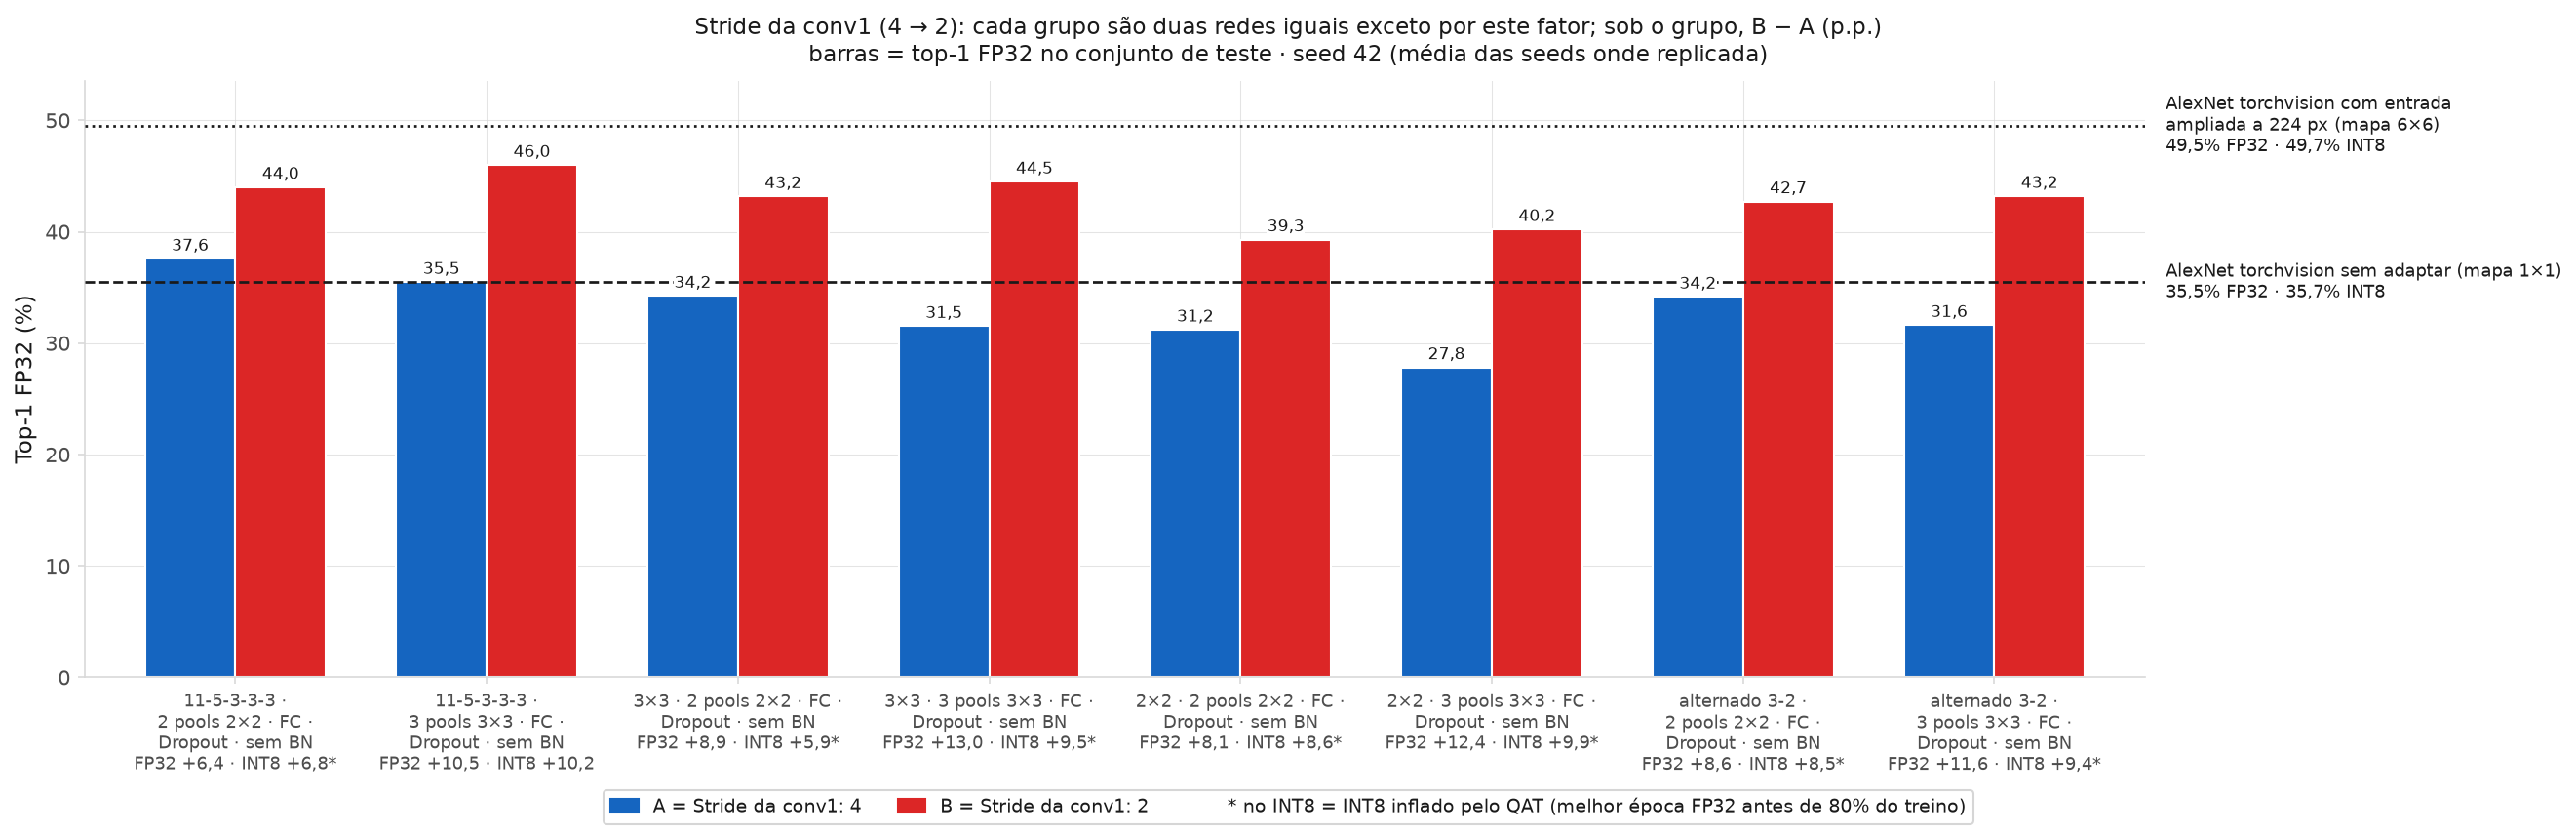
\includegraphics[width=\textwidth]{phase_11_kernel_size_comparison/05_conv1_stride.png}
\caption{O stride da conv1 pesa mais que o kernel. Reduzir o stride de 4 para 2 (vermelho) ganha em todos os oito pares. As linhas horizontais
são as referências da AlexNet sem adaptação e com a imagem ampliada para 224 px.}
\label{fig:stride}
\end{figure*}

\subsection{Quanto custa restringir o kernel?}
\label{sec:custo}

Custa pouco. A Figura~\ref{fig:pares} e a Tabela~\ref{tab:fatores_efeito} colocam o kernel ao lado dos outros fatores. Trocar 11-5-3-3-3 por
3\by3 custa 1,5 p.p., com IC de $-$3,3 a $+$0,7, que inclui o zero, e reduz os MACs em 25\%. Trocar 3\by3 por 2\by2 custa 2,5 p.p. (IC de
$-$3,7 a $-$1,1) e reduz os MACs em 54\%. O alternado 3-2 empata com o 3\by3 e usa 24\% menos MACs. Já BatchNorm, Dropout e pré-treino mudam
a acurácia em 4 a 5 p.p.

\begin{figure*}[!t]
\centering
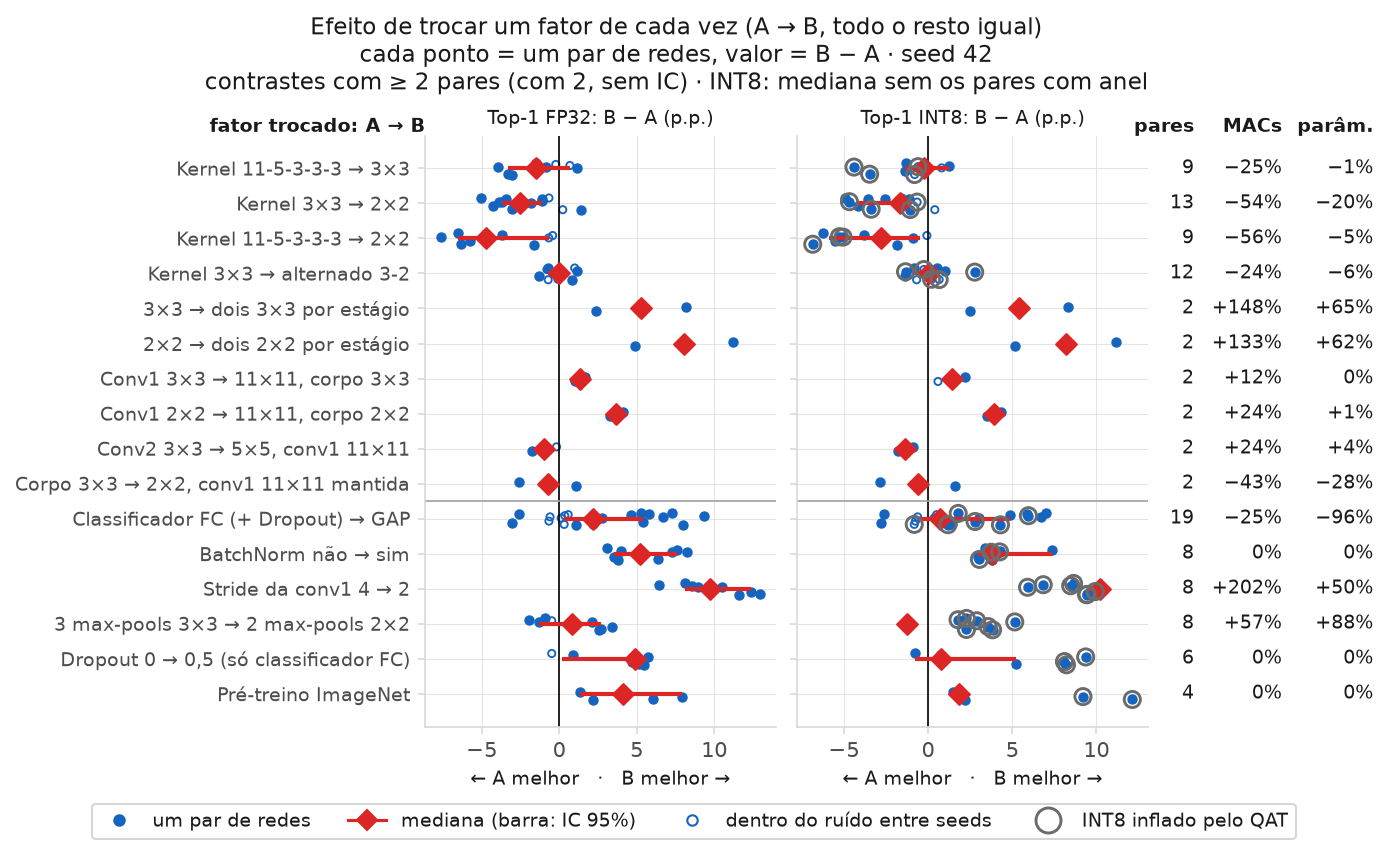
\includegraphics[width=0.86\textwidth,trim=0 0 0 91.2,clip]{phase_11_kernel_size_comparison/11_factorial_matched_pairs.png}
\caption{Efeito de trocar um fator de cada vez, em FP32 e em INT8 (seed 42, comparações com 3 ou mais pares). Cada ponto é um par de redes, e
o losango é a mediana. As quatro primeiras linhas são de kernel: note como ficam perto do zero em relação às outras. Pontos vazados estão
dentro da variação entre seeds, e os cinzas têm INT8 inflado pelo QAT.}
\label{fig:pares}
\end{figure*}

\begin{table*}[!t]
\caption{Efeito de cada fator: mediana de B $-$ A entre pares de redes iguais no resto (seed 42)}
\label{tab:fatores_efeito}
\centering
\small
\begin{tabular}{@{}lccccccc@{}}
\toprule
\textbf{A $\rightarrow$ B} & \textbf{Pares} & \textbf{FP32 (p.p.)} & \textbf{IC 95\%} & \textbf{B acima de A} & \textbf{INT8 (p.p.)} & \textbf{MACs} & \textbf{Parâmetros} \\
\midrule
Kernel 11-5-3-3-3 $\rightarrow$ 3\by3 & 9 & $-$1,5 & [$-$3,3; $+$0,7] & 2 de 9 & $-$0,8 & $-$25\% & $-$1\% \\
Kernel 3\by3 $\rightarrow$ 2\by2 & 13 & $-$2,5 & [$-$3,7; $-$1,1] & 2 de 13 & $-$1,7 & $-$54\% & $-$20\% \\
Kernel 11-5-3-3-3 $\rightarrow$ 2\by2 & 9 & $-$4,7 & [$-$6,5; $-$0,7] & 0 de 9 & $-$5,1 & $-$56\% & $-$5\% \\
Kernel 3\by3 $\rightarrow$ alternado 3-2 & 12 & 0,0 & [$-$0,7; $+$0,5] & 6 de 12 & $+$0,1 & $-$24\% & $-$6\% \\
3\by3 $\rightarrow$ dois 3\by3 por estágio & 2 & $+$5,3 & [$+$2,4; $+$8,1] & 2 de 2 & $+$5,4 & $+$148\% & $+$65\% \\
2\by2 $\rightarrow$ dois 2\by2 por estágio & 2 & $+$8,0 & [$+$4,9; $+$11,2] & 2 de 2 & $+$8,2 & $+$133\% & $+$62\% \\
Conv1 3\by3 $\rightarrow$ 11\by11, corpo 3\by3 & 2 & $+$1,3 & [$+$1,0; $+$1,6] & 2 de 2 & $+$1,4 & $+$12\% & 0\% \\
Conv1 2\by2 $\rightarrow$ 11\by11, corpo 2\by2 & 2 & $+$3,7 & [$+$3,3; $+$4,1] & 2 de 2 & $+$3,9 & $+$24\% & $+$1\% \\
FC + Dropout $\rightarrow$ GAP & 19 & $+$2,1 & [$+$0,3; $+$5,4] & 15 de 19 & $+$1,4 & $-$25\% & $-$96\% \\
BatchNorm: não $\rightarrow$ sim & 8 & $+$5,2 & [$+$3,5; $+$7,6] & 8 de 8 & $+$3,8 & 0\% & 0\% \\
Stride da conv1: 4 $\rightarrow$ 2 & 8 & $+$9,7 & [$+$8,1; $+$12,4] & 8 de 8 & $+$9,0 & $+$202\% & $+$50\% \\
3 \textit{max-pools} 3\by3 $\rightarrow$ 2 \textit{max-pools} 2\by2 & 8 & $+$0,8 & [$-$1,3; $+$2,7] & 4 de 8 & $+$2,6 & $+$57\% & $+$88\% \\
Dropout: 0 $\rightarrow$ 0,5 (só FC) & 6 & $+$4,9 & [$+$0,2; $+$5,6] & 5 de 6 & $+$6,7 & 0\% & 0\% \\
Pré-treino ImageNet & 4 & $+$4,1 & [$+$1,4; $+$7,9] & 4 de 4 & $+$5,7 & 0\% & 0\% \\
\bottomrule
\end{tabular}
\end{table*}

O custo depende do classificador, como mostra a Figura~\ref{fig:grade}. Com GAP e BatchNorm, o 3\by3 nem chega a perder: fica em 53,81\%,
contra 53,07\% do 11-5-3-3-3 (3 seeds cada), e o alternado 3-2 chega a 54,58\%. Nessa configuração, o 2\by2 custa 1,2 p.p. em relação ao
3\by3 (52,58\%). Com FC, Dropout e BatchNorm, a mesma troca custa 5,1 p.p. (seed 42).

\begin{figure*}[!t]
\centering
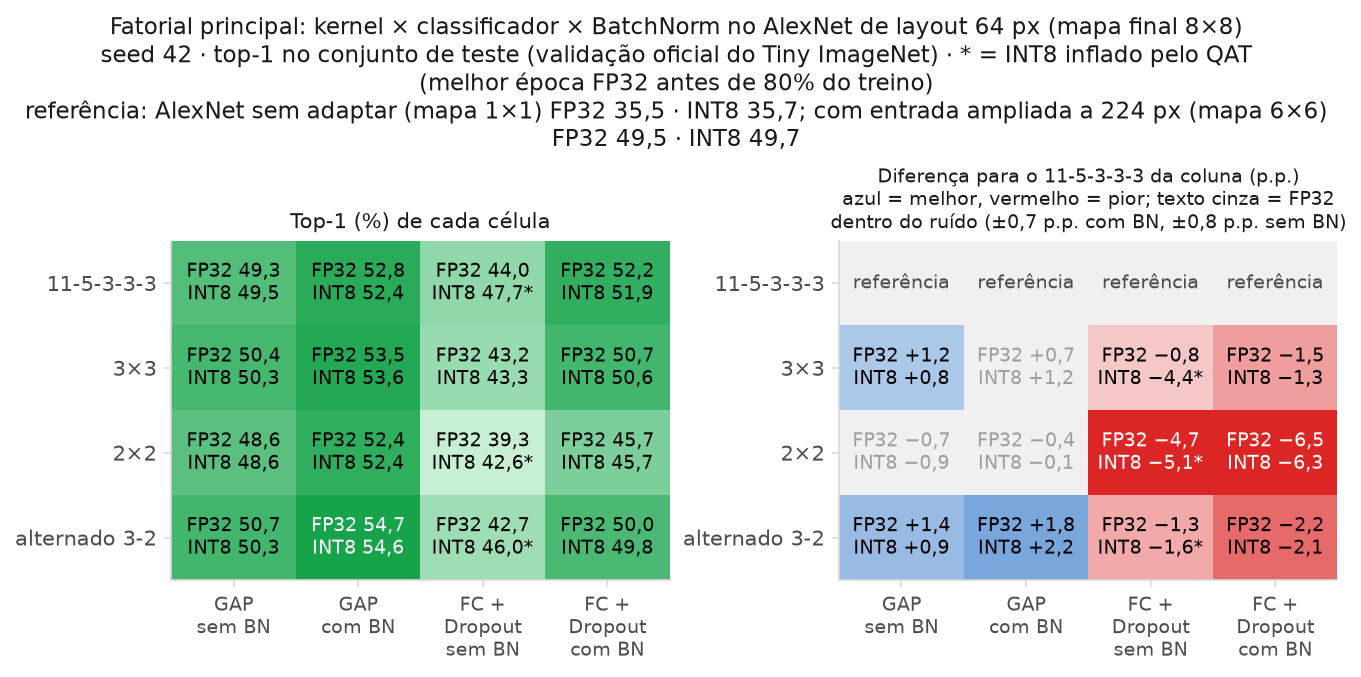
\includegraphics[width=\textwidth,trim=0 0 0 56.6,clip]{phase_11_kernel_size_comparison/14_main_factorial_grid.png}
\caption{Kernel, classificador e BatchNorm na AlexNet de layout 64 px. À esquerda, a acurácia de cada combinação; à direita, a diferença para o
11-5-3-3-3 da mesma coluna. Com GAP (duas primeiras colunas), os kernels pequenos ficam perto do original ou acima dele. Cinza: dentro da variação entre seeds; asterisco: INT8 inflado pelo QAT. Para comparar: a AlexNet sem adaptação fica em 35,5\% em FP32, e com imagem ampliada para 224 px, em 49,5\%. Seed 42.}
\label{fig:grade}
\end{figure*}

A Figura~\ref{fig:vgg} repete a comparação na VGG16. Com GAP e BatchNorm, o 2\by2 custa 2,4 p.p. (56,84\% contra 59,27\%, 3 seeds cada).
Com FC e Dropout, esse custo desaparece (59,17\% contra 58,83\%, 3 seeds). Com FC sem Dropout, o 2\by2 fica 1,1 p.p. abaixo (uma seed). Na ResNet-18, o 2\by2 custa 1,0 p.p. em relação ao 3\by3 (3 seeds).

\begin{figure*}[!t]
\centering
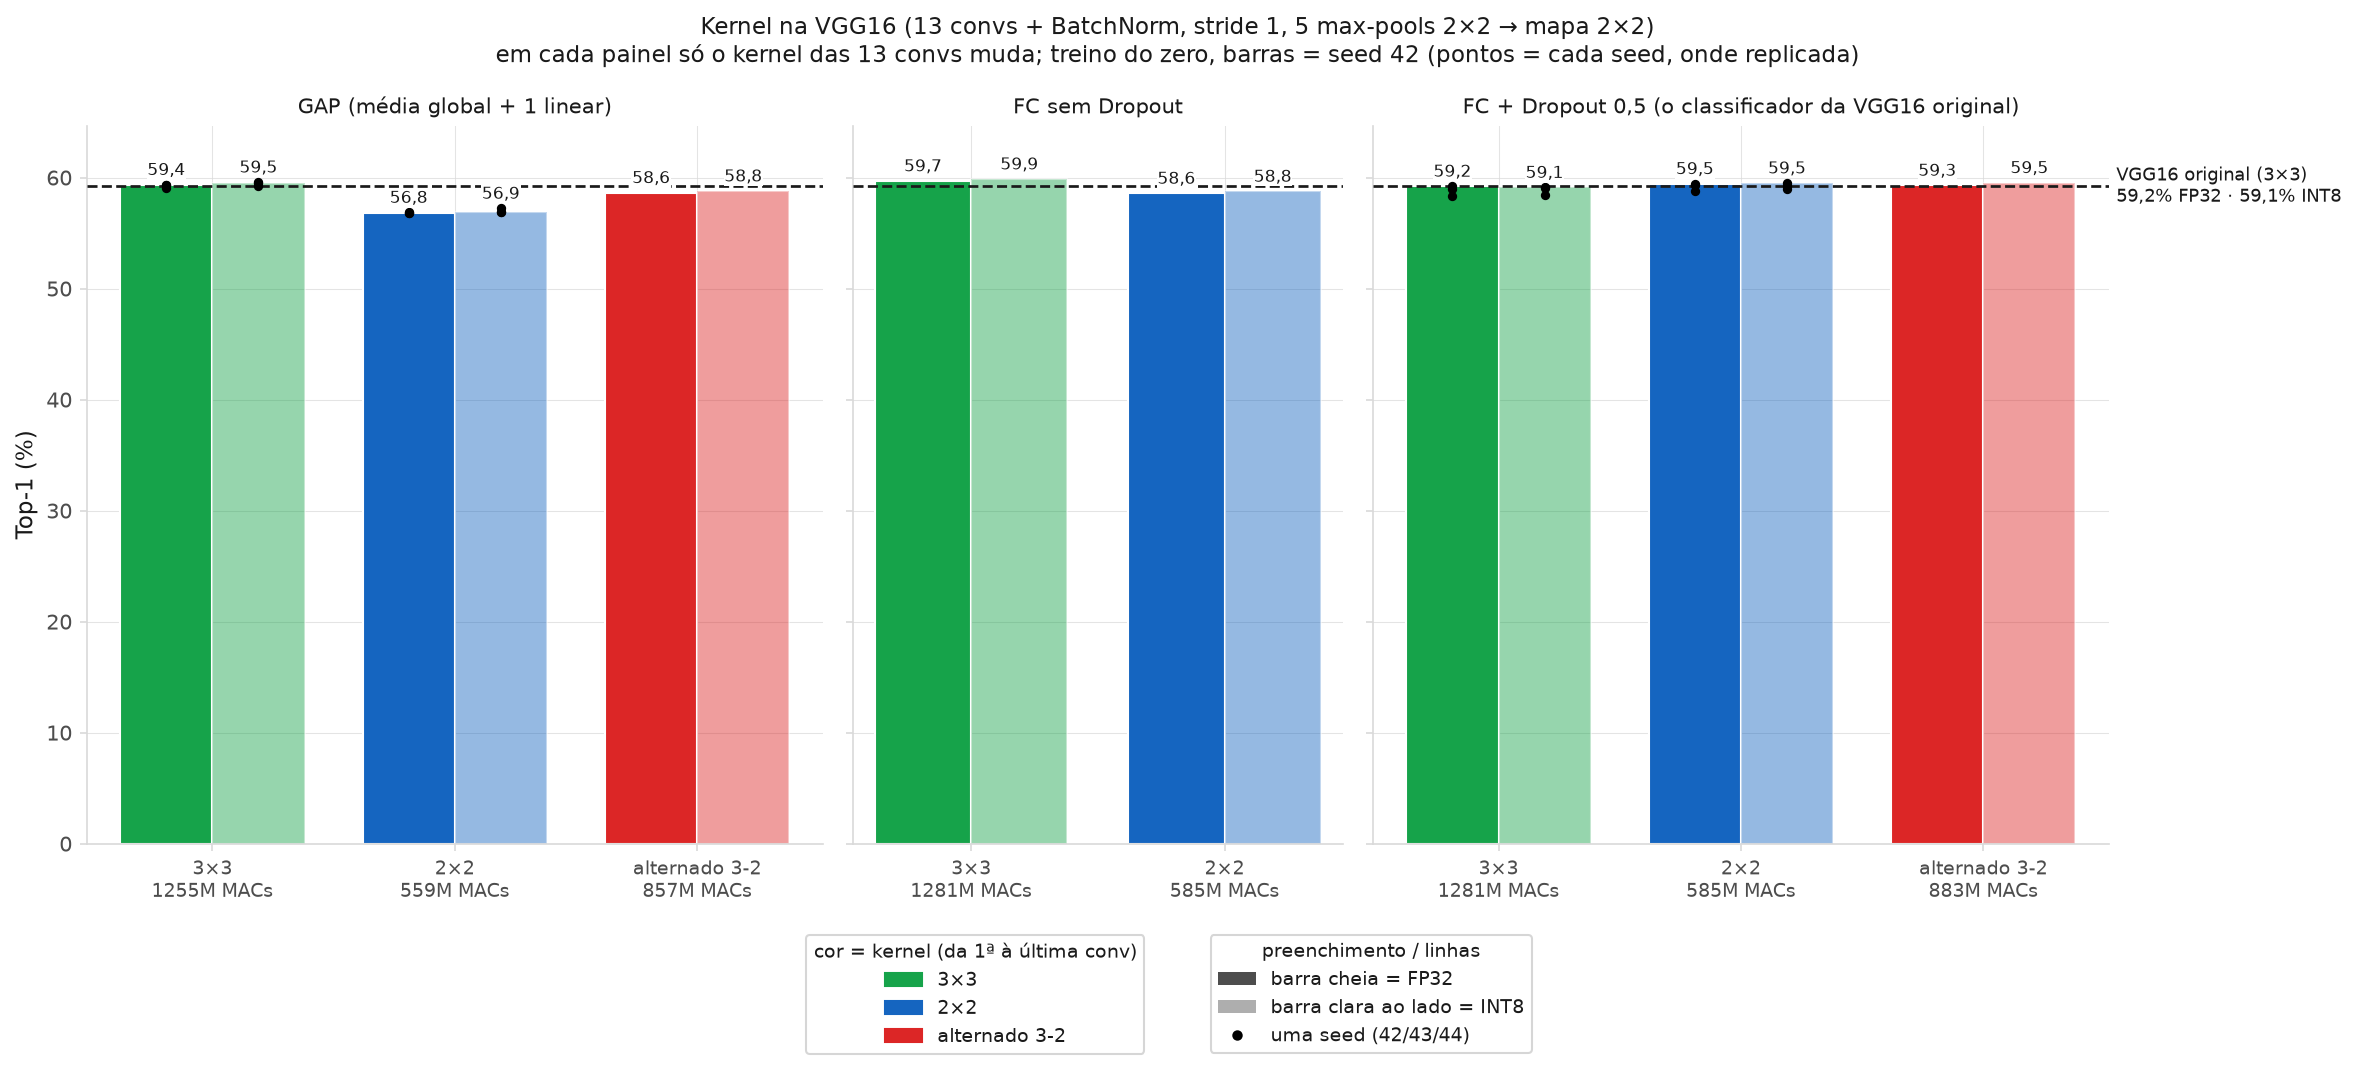
\includegraphics[width=0.86\textwidth]{phase_11_kernel_size_comparison/03_kernel_vgg16.png}
\caption{Kernel na VGG16. Em cada painel, só o kernel das 13 convoluções muda. O 2\by2 perde com GAP e, por menos, com FC sem Dropout (uma seed). Com FC + Dropout, empata.}
\label{fig:vgg}
\end{figure*}

\subsection{O 2\by2 perde pelo kernel ou pelo custo?}
\label{sec:controles}

Pelo custo. Para separar as duas coisas, alargamos a rede 2\by2 até ela gastar o mesmo que a 3\by3 e estreitamos a 3\by3 até ela gastar
o mesmo que a 2\by2 (Figura~\ref{fig:controles}a). Com o mesmo custo, as redes empatam: 53,83\% contra 53,81\% com 167M de MACs, e 52,58\%
contra 52,59\% com 75M (3 seeds cada).

Kernels maiores, por outro lado, não compram acurácia. Com 5\by5 em todas as convoluções, a rede custa 2,8 vezes o 3\by3 e chega a 49,25\%, ou
4,6 p.p. abaixo dele (3 seeds, Figura~\ref{fig:controles}b). Com GAP e BatchNorm, gastar mais só compensou como largura, não como kernel maior.
A exceção é o classificador FC + Dropout, em que o 5\by5 chega a 52,14\% (uma seed), perto dos 52,23\% do 11-5-3-3-3.

\begin{figure*}[!t]
\centering
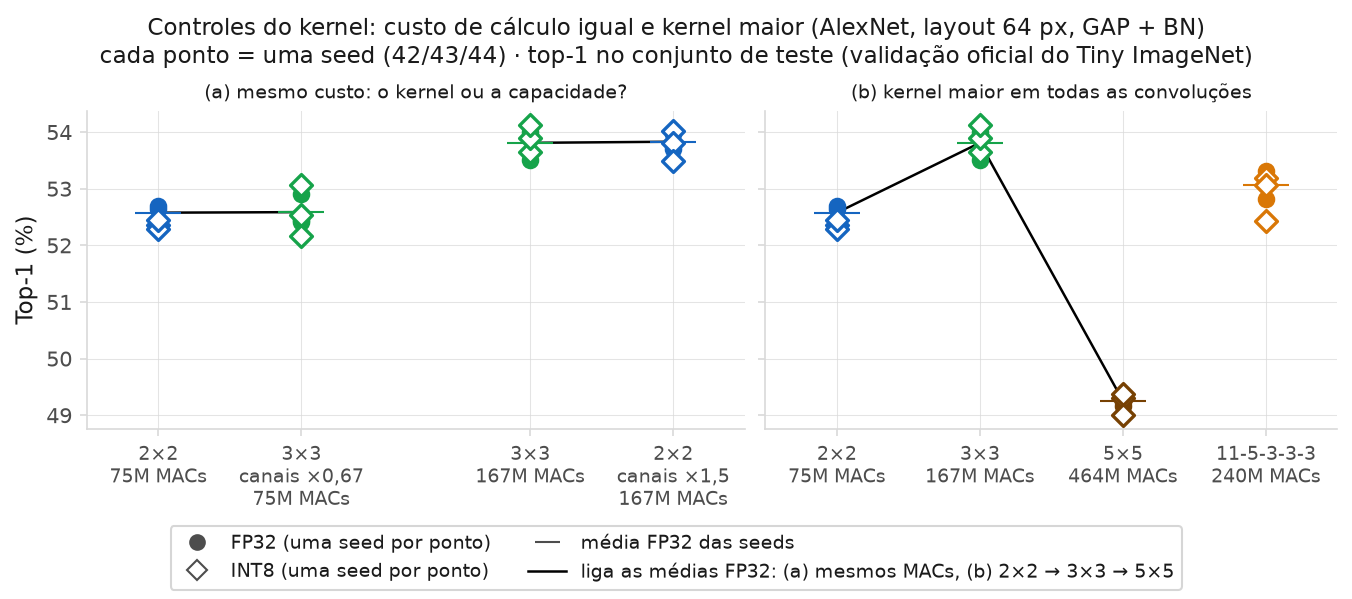
\includegraphics[width=0.72\textwidth]{phase_11_kernel_size_comparison/26_kernel_controls.png}
\caption{(a) Com o mesmo custo em MACs, 2\by2 e 3\by3 empatam. (b) Um kernel maior não ajuda: o 5\by5 custa mais e fica bem abaixo do 3\by3.
Cada ponto é uma seed. AlexNet de layout 64 px, GAP e BatchNorm.}
\label{fig:controles}
\end{figure*}

A Figura~\ref{fig:blocos} mostra onde o 2\by2 custa na VGG16. Colocá-lo em um único bloco quase não muda nada: 59,54\%, 59,34\%, 59,05\% e
59,18\% nos blocos 1, 2, 3 e 5 (3 seeds), contra 59,27\% com 3\by3 em todos. O bloco 4 é o único que parece custar algo (58,56\%). Essa
diferença de 0,71 p.p. ainda está dentro da variação, mas se repete nas três seeds. A perda maior só aparece quando todos os blocos usam 2\by2.

\begin{figure*}[!t]
\centering
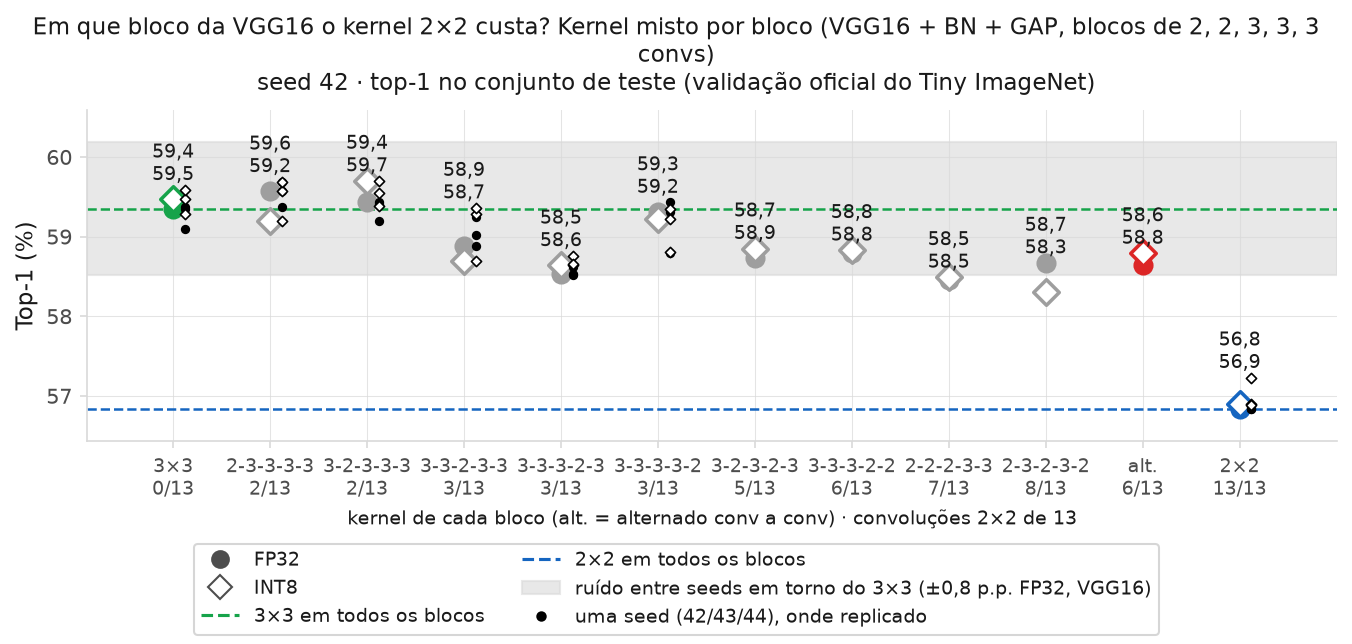
\includegraphics[width=\textwidth]{phase_11_kernel_size_comparison/24_vgg_kernel_blocks.png}
\caption{VGG16 com um kernel por bloco. Os padrões leem-se bloco a bloco: 3-3-3-2-3 tem 2\by2 só no bloco 4. A faixa cinza é a variação entre
seeds em torno do 3\by3. Só a rede com 2\by2 em todos os blocos sai claramente dela.}
\label{fig:blocos}
\end{figure*}

\subsection{Dá para recuperar a perda sem um corpo de kernel grande?}
\label{sec:recuperar}

Sim, de duas formas. A primeira é manter só a conv1 11\by11 e usar 2\by2 no resto (Figura~\ref{fig:conv1}). Essa rede chega a 55,93\% em FP32 e
56,11\% em INT8 (3 seeds) com 98M de MACs. É mais que o 3\by3 (53,81\%, 167M) e que os kernels originais (53,07\%, 240M). Como a conv1 tem stride
2, ela já ficaria fora de um acelerador de Winograd de qualquer forma, então o kernel grande não tira nada dele.

\begin{figure*}[!t]
\centering
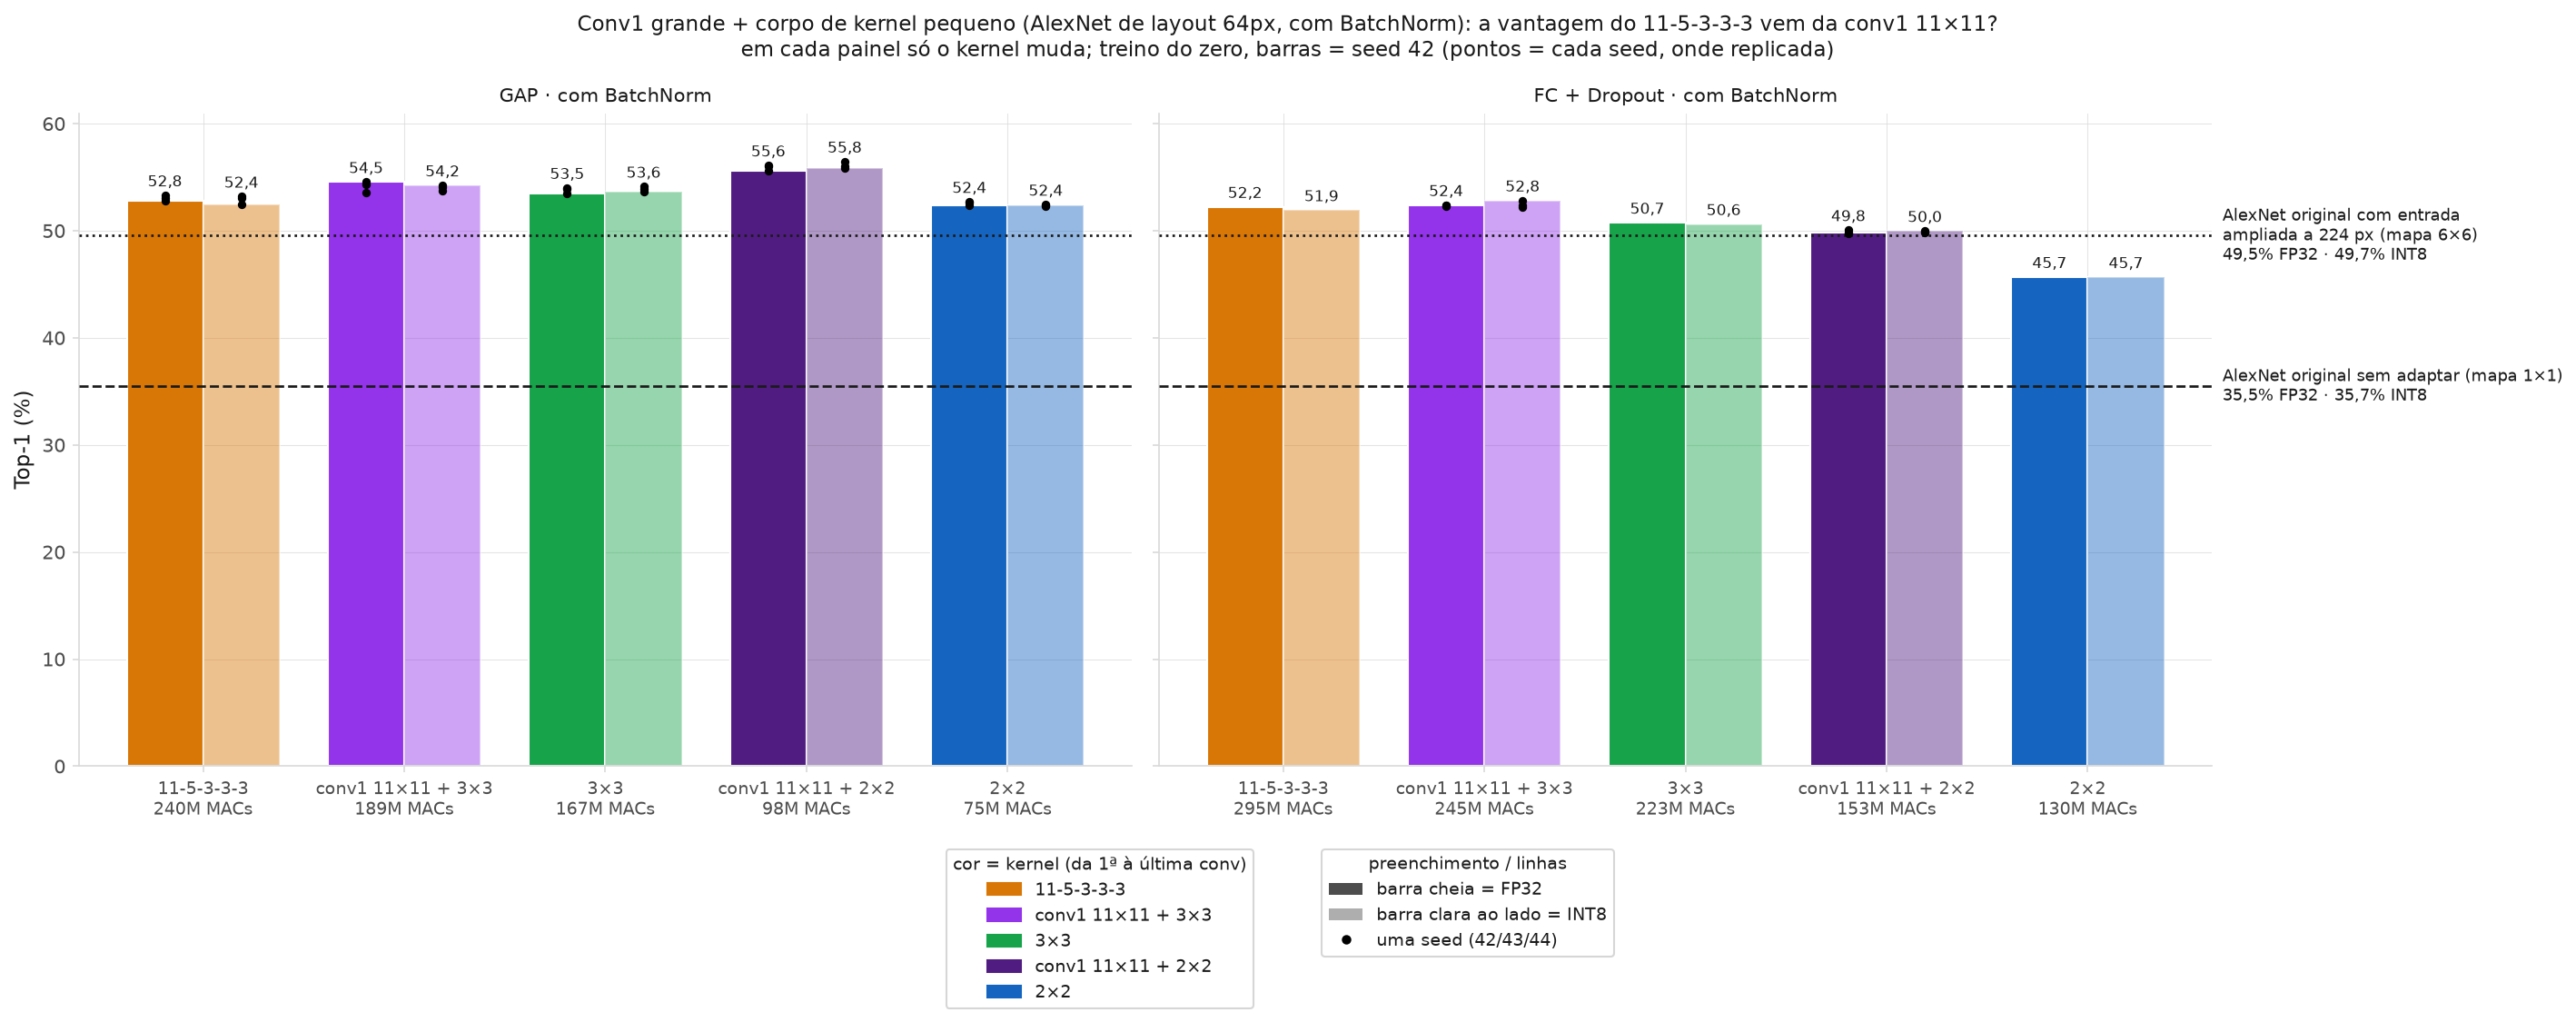
\includegraphics[width=\textwidth]{phase_11_kernel_size_comparison/27_large_stem.png}
\caption{Conv1 grande com corpo de kernel pequeno. Com GAP (à esquerda), a conv1 11\by11 com corpo 2\by2 é a melhor das cinco e a segunda mais
barata. Barra cheia: FP32; barra clara: INT8; pontos: cada seed.}
\label{fig:conv1}
\end{figure*}

A segunda forma é usar duas convoluções pequenas por estágio. Isso ganha 5,3 p.p. com 3\by3 e 8,0 p.p. com 2\by2, com 130 a 150\% mais MACs
(Tabela~\ref{tab:fatores_efeito}, dois pares cada). Com GAP e BatchNorm, a rede 2\by2 empilhada (57,25\%, 201M) fica até acima da 3\by3 empilhada
(55,87\%, 451M), com uma seed cada.

O campo receptivo efetivo ajuda a entender a diferença \cite{luo2016understanding}. A Figura~\ref{fig:erf} mostra quanto cada pixel influencia o
centro da última camada. Empilhar amplia a região usada: a área com metade da influência vai de 17,8\% para 29,8\% da imagem no 2\by2, e de 23,5\% para
33,1\% no 3\by3. Já a conv1 11\by11 quase não amplia essa área (18,5\% contra 17,8\%), embora melhore a acurácia. Seu ganho, portanto, não parece vir
de enxergar mais da imagem. Não testamos a causa.

\begin{figure*}[!t]
\centering
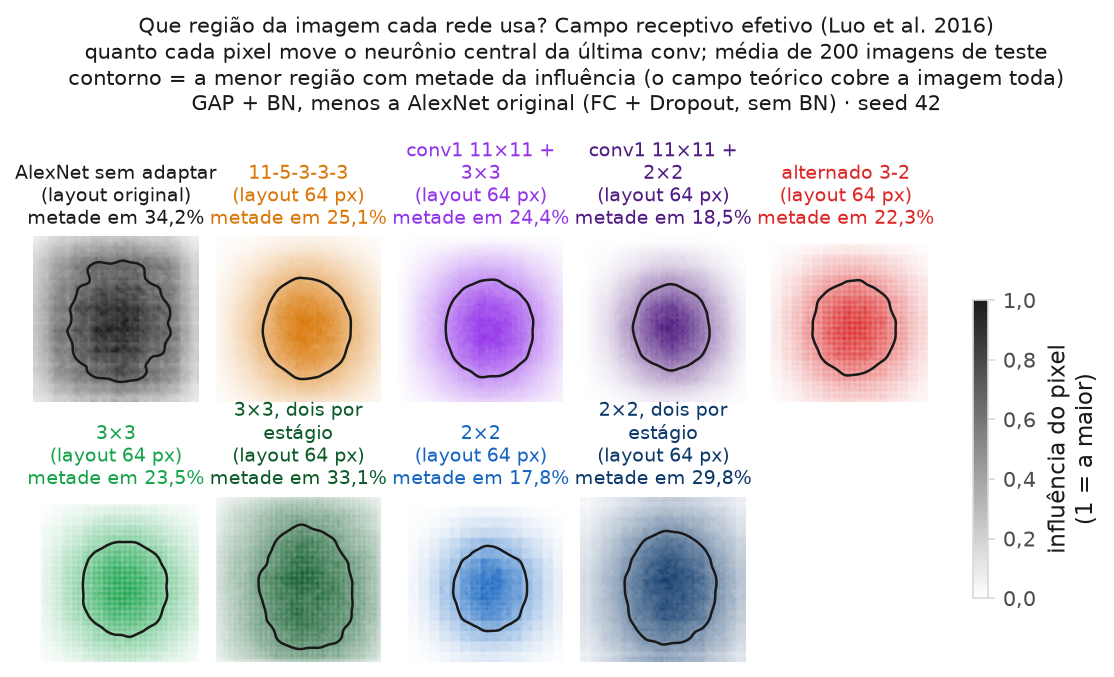
\includegraphics[width=0.8\textwidth]{phase_11_kernel_size_comparison/22_effective_receptive_field.png}
\caption{Que região da imagem cada rede usa (média de 200 imagens de teste, seed 42). O contorno marca a menor região com metade da influência.
Compare, na segunda linha, 2\by2 com 2\by2 empilhado e 3\by3 com 3\by3 empilhado.}
\label{fig:erf}
\end{figure*}

\subsection{A quantização INT8 atrapalha?}
\label{sec:int8}

Quase nada, e o kernel não muda isso (Figura~\ref{fig:int8}). Nos 126 treinos do estudo principal sem a marca de melhor época cedo, a diferença
entre INT8 e FP32 vai de $-$0,38 a $+$0,58 p.p., com mediana de $+$0,04 p.p. Nos 26 treinos marcados, ela vai de $+$0,56 a $+$6,69 p.p. Esse aumento não
é efeito da quantização: o QAT continua treinando uma rede que ainda não tinha terminado de convergir, agora com uma taxa de aprendizado baixa.
No estudo de combinações, nenhum treino recebeu a marca, e a diferença vai de $-$0,44 a $+$0,77 p.p.

\begin{figure*}[!t]
\centering
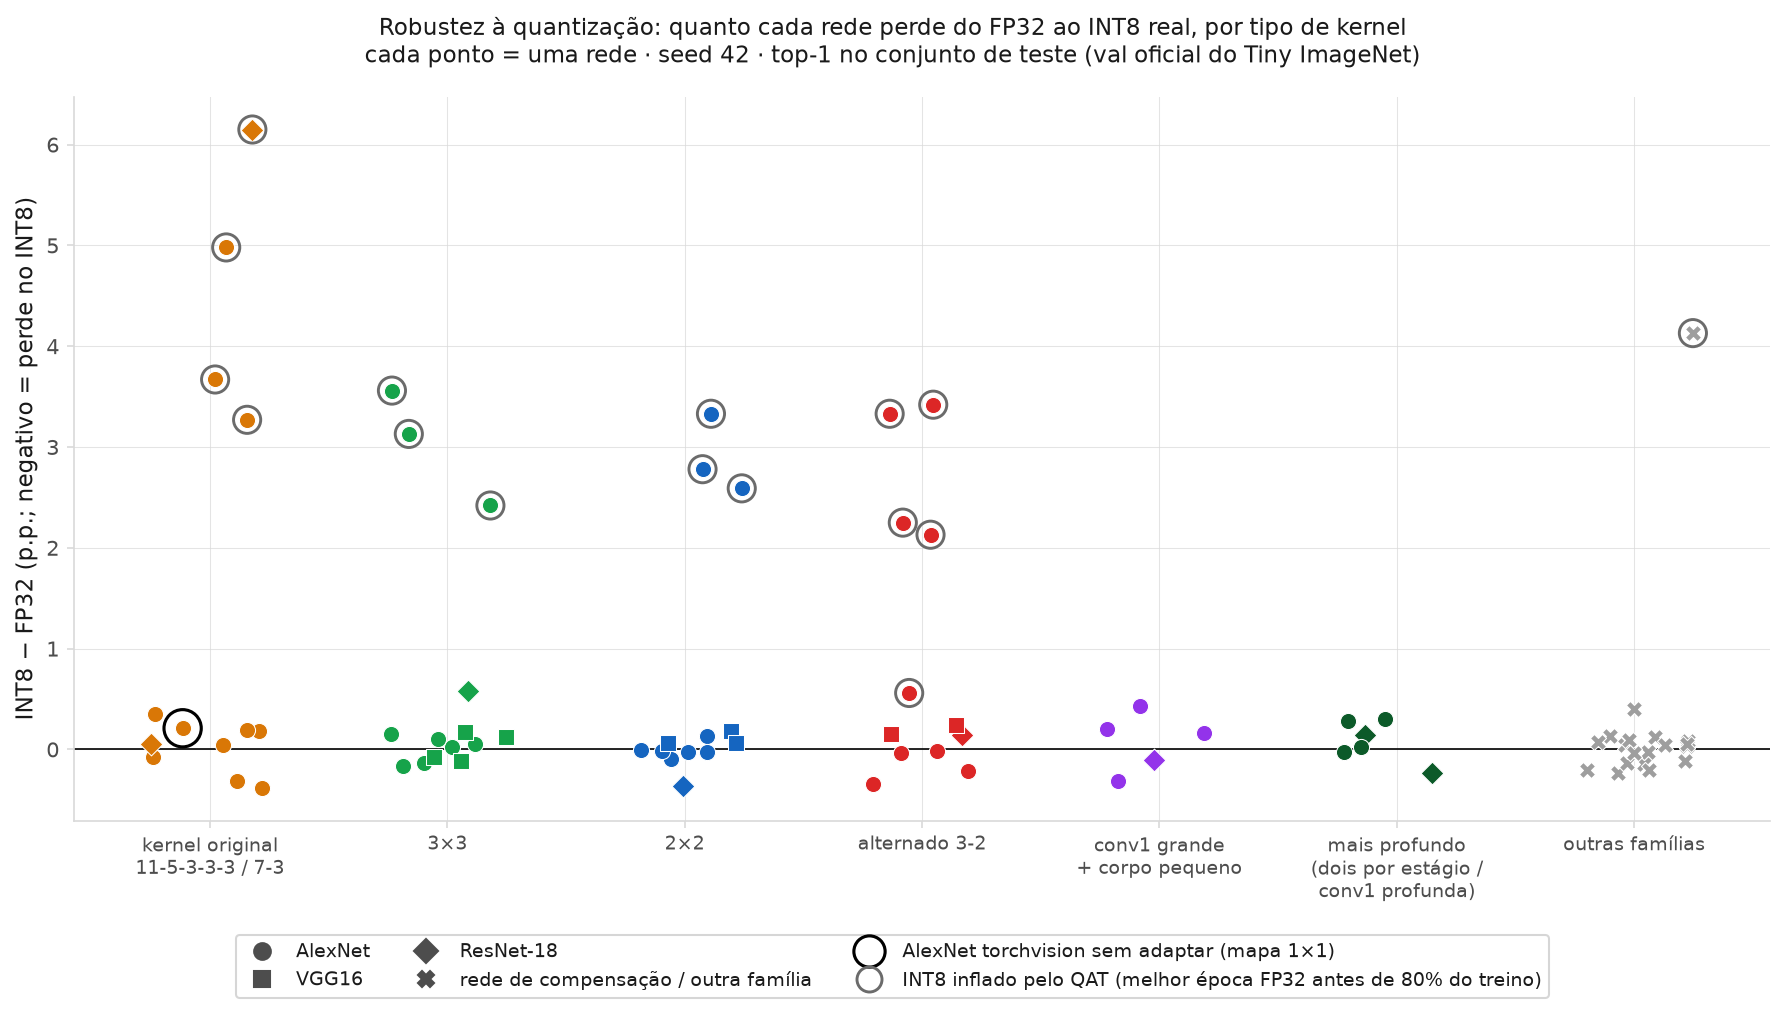
\includegraphics[width=0.8\textwidth]{phase_11_kernel_size_comparison/16_quantization_robustness.png}
\caption{Quanto cada rede muda do FP32 para o INT8, por tipo de kernel (seed 42). Sem a marca do anel, todas as redes ficam perto de zero, seja qual
for o kernel. Os pontos altos, com anel, são treino extra do QAT.}
\label{fig:int8}
\end{figure*}

Acurácia igual, porém, não quer dizer respostas iguais \cite{hooker2019what}. A Figura~\ref{fig:flips} conta as imagens que mudam entre certo e errado.
A maioria das redes troca de 2\% a 7\% das imagens de teste, em quantidades parecidas nas duas direções. As redes marcadas chegam, em geral, a 9--14\%,
e quase sempre ganham no saldo.

\begin{figure*}[!t]
\centering
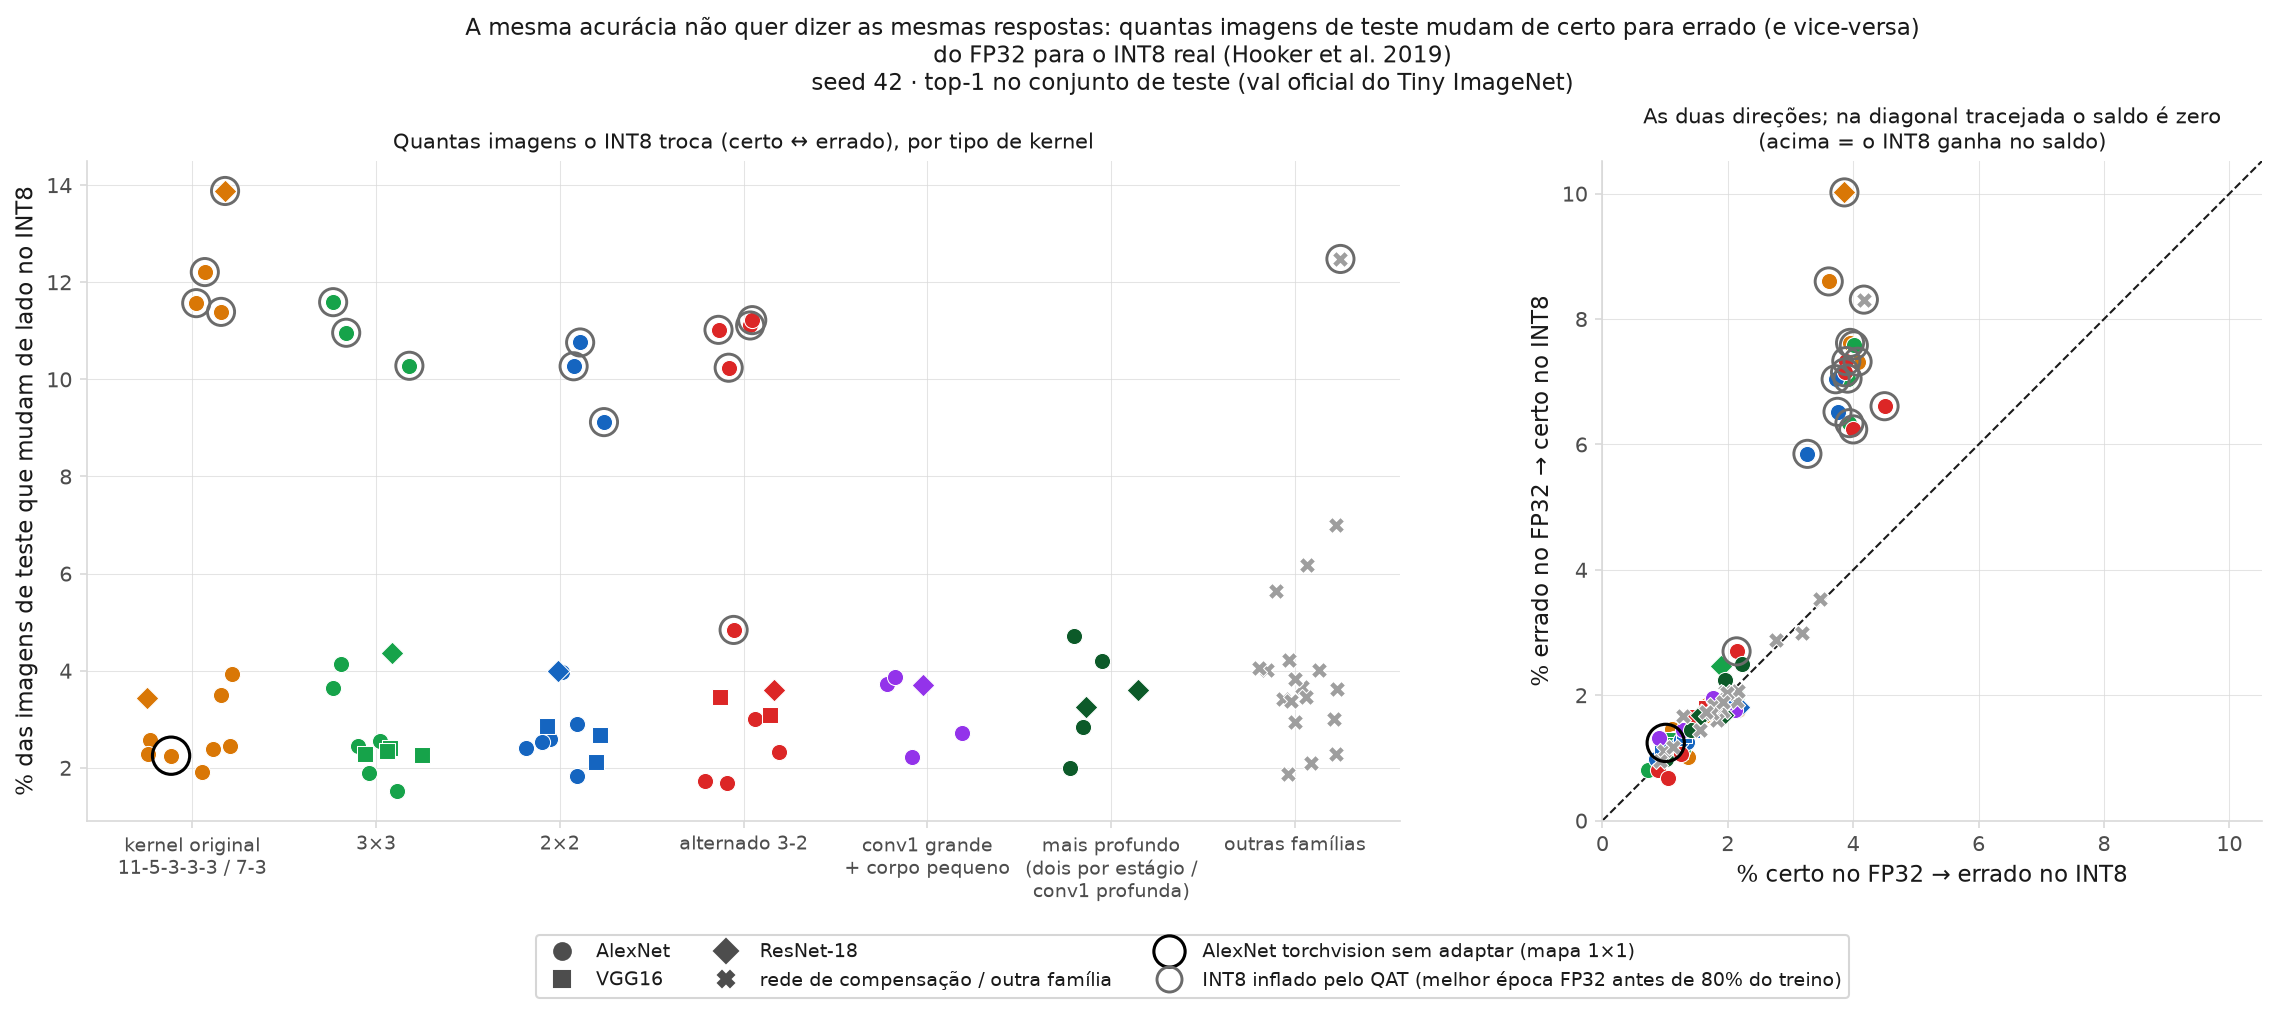
\includegraphics[width=0.86\textwidth]{phase_11_kernel_size_comparison/20_int8_prediction_flips.png}
\caption{Imagens que mudam entre certo e errado do FP32 para o INT8 (seed 42). À direita, sobre a diagonal, o saldo é zero. Só as redes com anel ficam
claramente acima dela.}
\label{fig:flips}
\end{figure*}

Há uma exceção a acompanhar: a MobileNetV2 pré-treinada. Com ajuste fino, ela perde 1,49 p.p. (taxa de aprendizado 10$^{-4}$) e 1,16 p.p. (10$^{-3}$) do
FP32 para o INT8, quase tudo já no QAT. Fora ela, nenhum treino sem marca dos dois primeiros estudos perde mais de 0,38 p.p. Ela é a única rede
pré-treinada com convoluções \textit{depthwise}, mas não investigamos a causa.

\subsection{Quanto da rede cabe em um acelerador Winograd?}
\label{sec:hardware}

As Figuras~\ref{fig:pareto} e~\ref{fig:winograd} comparam acurácia e custo. A linha tracejada liga as redes que nenhuma outra supera em acurácia e
custo ao mesmo tempo. Na parte barata, ela passa por redes de compensação, como a Bottleneck. Na parte intermediária, passa pela conv1 11\by11 com corpo
2\by2 e pela 2\by2 empilhada. Na parte cara, passa pela VGG16.

\begin{figure*}[!t]
\centering
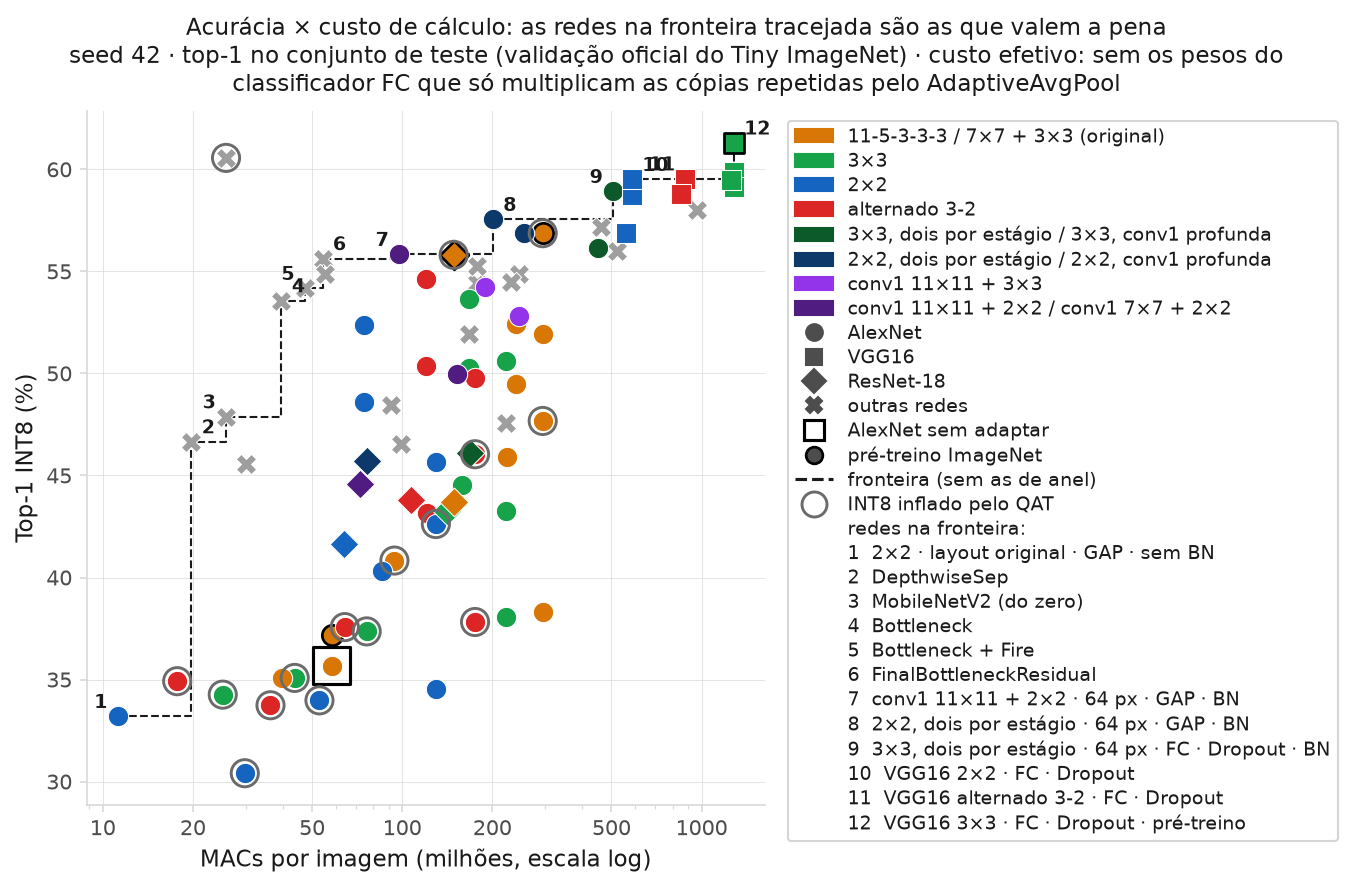
\includegraphics[width=0.86\textwidth]{phase_11_kernel_size_comparison/13_pareto_accuracy_cost.png}
\caption{Acurácia INT8 e custo em MACs (estudo principal, seed 42). A linha tracejada liga as redes que nenhuma outra supera nos dois critérios ao mesmo
tempo; as redes com anel ficam fora dela, porque seu INT8 está inflado pelo QAT.}
\label{fig:pareto}
\end{figure*}

\begin{figure*}[!t]
\centering
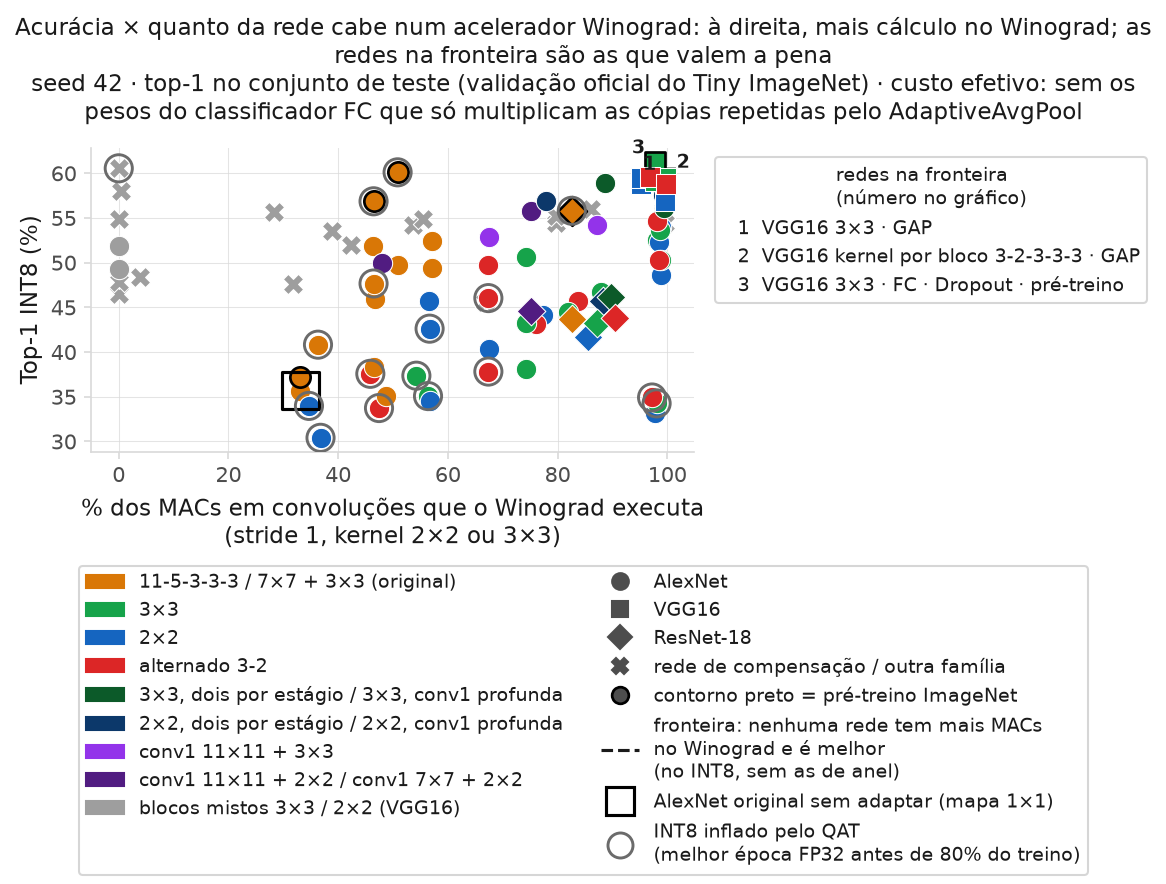
\includegraphics[width=0.86\textwidth]{phase_11_kernel_size_comparison/30_winograd_eligible.png}
\caption{Acurácia INT8 e parcela dos MACs em convoluções que um acelerador Winograd pode executar (stride 1, kernel 2\by2 ou 3\by3, sem grupos). Sem contar as redes com anel, as
mais precisas, no canto superior direito, cabem quase inteiras. A conta usa só a geometria das camadas.}
\label{fig:winograd}
\end{figure*}

Barato não significa adequado para Winograd. A Tabela~\ref{tab:winograd} mostra a parcela dos MACs em convoluções densas de stride 1, com kernel 2\by2 ou
3\by3. As AlexNets de kernel pequeno e a VGG16 ficam perto de 100\%. A TinyMobileNetV2 e a MobileNetV2 ficam em torno de zero, e a
FinalBottleneckResidual, em 28\%. Essas redes são eficientes, mas gastam a maior parte do cálculo em convoluções 1\by1, \textit{depthwise} ou de stride maior que 1, que o
acelerador não aproveita \cite{souza2026relatorio}. A busca por uma rede eficiente e a busca por uma rede para Winograd levam, portanto, a escolhas diferentes.

\begin{table}[!t]
\caption{Acurácia, custo e parcela dos MACs em convoluções densas de stride 1 com kernel 2\by2 ou 3\by3 (seed 42)}
\label{tab:winograd}
\centering
\footnotesize
\setlength{\tabcolsep}{3pt}
\begin{tabular}{@{}lccccc@{}}
\toprule
\textbf{Rede} & \textbf{FP32} & \textbf{INT8} & \textbf{Parâm.} & \textbf{MACs} & \textbf{Winograd} \\
 & \textbf{(\%)} & \textbf{(\%)} & \textbf{(M)} & \textbf{(M)} & \textbf{(\%)} \\
\midrule
2\by2 + atalho, stride 1 & 60,75 & 60,46 & 2,52 & 862 & 92,9 \\
2\by2 empilhada, stride 1 & 60,35 & 60,79 & 2,33 & 803 & 99,6 \\
VGG16 3\by3 & 59,35 & 59,47 & 14,82 & 1255 & 99,8 \\
TinyMobileNetV2 & 57,96 & 58,00 & 1,51 & 969 & 0,4 \\
2\by2 empilhada & 57,25 & 57,55 & 2,33 & 201 & 99,2 \\
SmallKernel + BN & 57,20 & 57,17 & 1,60 & 461 & 99,7 \\
FinalBottleneckResidual & 55,83 & 55,63 & 0,57 & 54 & 28,3 \\
Conv1 11\by11 + corpo 2\by2 & 55,64 & 55,84 & 1,08 & 98 & 75,2 \\
FireBypass & 55,19 & 55,27 & 0,52 & 178 & 79,7 \\
Fire & 54,57 & 54,44 & 0,52 & 178 & 79,7 \\
Bottleneck & 53,71 & 53,57 & 0,39 & 40 & 38,8 \\
3\by3 & 53,50 & 53,65 & 2,30 & 167 & 98,7 \\
11-5-3-3-3 & 52,81 & 52,43 & 2,52 & 240 & 57,1 \\
2\by2 & 52,39 & 52,36 & 1,05 & 75 & 98,4 \\
MobileNetV2 (do zero) & 47,83 & 47,88 & 2,48 & 26 & 0,0 \\
DepthwiseSep & 46,53 & 46,66 & 0,31 & 20 & 0,0 \\
\bottomrule
\end{tabular}
\end{table}

\subsection{Os resultados valem em outras condições?}
\label{sec:robustez}

Sim. A Figura~\ref{fig:cenarios} resume os cenários. Trocar 3\by3 por 2\by2 custa de 0,7 a 2,4 p.p. em FP32 em todos eles e quase nada quando os MACs são
iguais. Com metade e com o dobro da taxa de aprendizado, a ordem das três redes testadas se mantém: 3\by3, 11-5-3-3-3 e 2\by2 (52,27\%, 52,15\% e 51,57\%;
54,22\%, 53,89\% e 53,22\%; uma seed cada). Trocar os kernels originais por 3\by3 empata ou melhora nos cenários com AlexNet. A exceção é a ResNet-18 ($-$0,95 p.p., uma seed).

\begin{figure*}[!t]
\centering
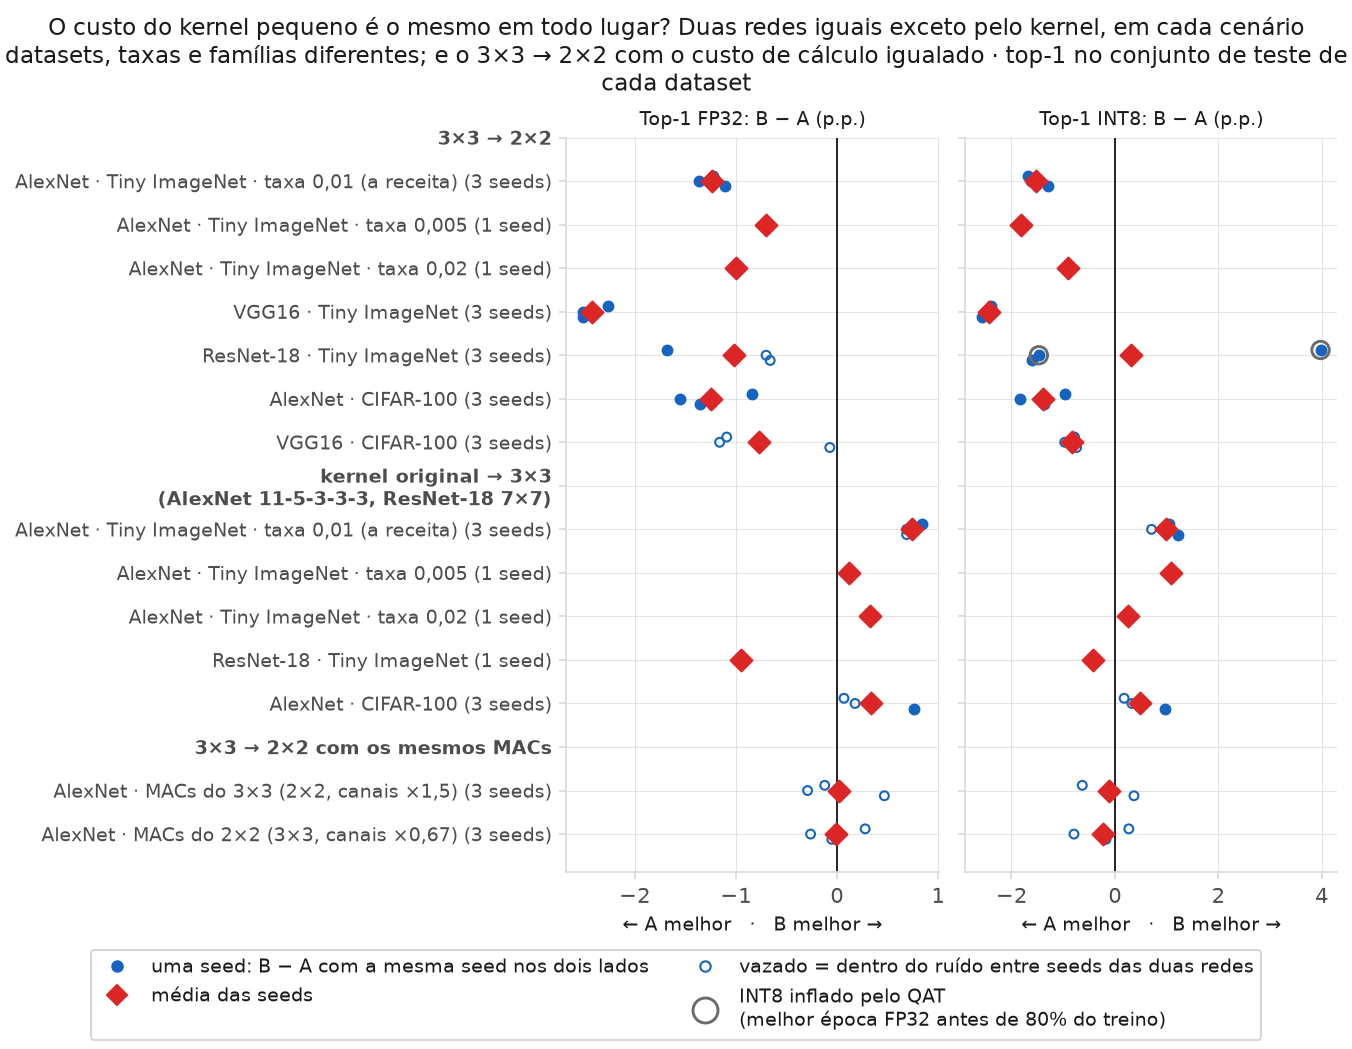
\includegraphics[width=0.74\textwidth]{phase_12_robustness/04_kernel_effect_everywhere.png}
\caption{O efeito do kernel em cada cenário: duas redes iguais exceto pelo kernel. O custo do 2\by2 aparece em todas as linhas do primeiro grupo e some no último, em que os MACs são iguais. O grupo do meio compara os kernels originais com 3\by3. Um ponto muito à direita no INT8 da ResNet-18 é um caso de INT8 inflado pelo QAT.}
\label{fig:cenarios}
\end{figure*}

No CIFAR-100 (3 seeds), a AlexNet com alternado 3-2 chega a 63,42\%, com 3\by3 a 63,34\%, com 11-5-3-3-3 a 63,00\% e com 2\by2 a 62,09\%. Na VGG16, o 3\by3 chega a
71,08\%, o alternado a 70,99\% e o 2\by2 a 70,31\%. A ordem dos kernels é a mesma do Tiny ImageNet nas duas famílias (Figura~\ref{fig:transferencia}), com $\tau$ de
Kendall igual a $+$1,00 \cite{kendall1938new}. Como são só quatro e três redes, e algumas ficam muito próximas, isso é um sinal de consistência, não uma prova.

\begin{figure*}[!t]
\centering
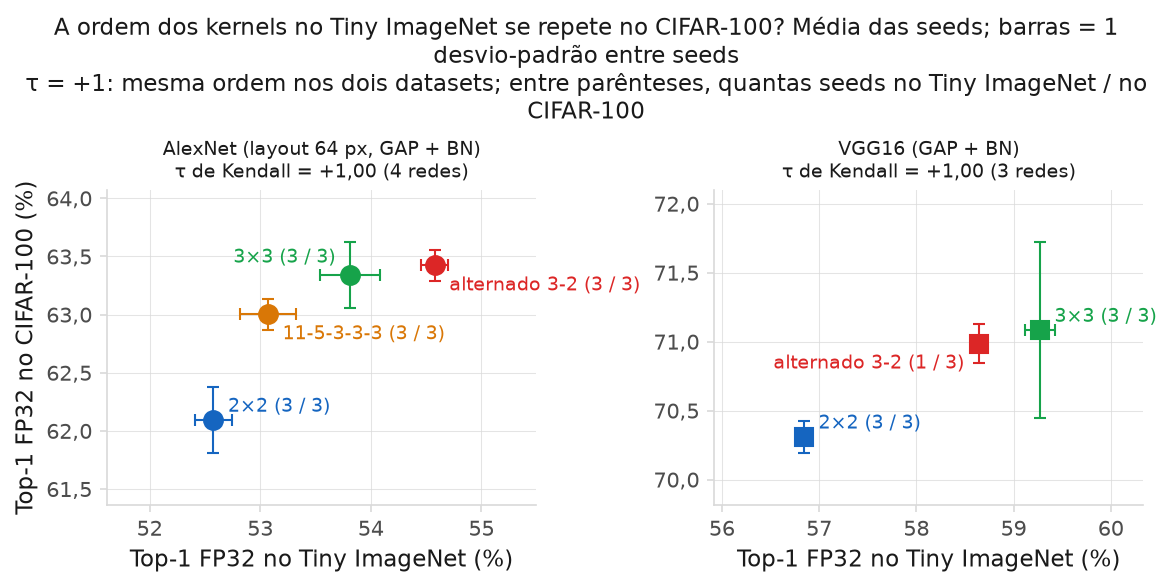
\includegraphics[width=0.72\textwidth]{phase_12_robustness/05_dataset_transfer.png}
\caption{A ordem dos kernels no Tiny ImageNet se repete no CIFAR-100. Cada ponto é a média das seeds, e as barras mostram um desvio-padrão entre seeds.}
\label{fig:transferencia}
\end{figure*}

O pré-treino merece uma observação. Com a receita única, a taxa de 0,01 apaga boa parte dele. Com ajuste fino de verdade \cite{li2020rethinking}, a taxa
de 10$^{-3}$ supera a de 10$^{-4}$ em todas as redes testadas em 64 px, e a VGG16 chega a 67,27\%. O ganho sobre a mesma rede treinada do zero vai de $+$5,5 a $+$14,9 p.p.
Esse resultado não responde à pergunta sobre kernels, porque os pesos pré-treinados só existem para os kernels originais de cada rede.

\subsection{Os ganhos se somam?}
\label{sec:combinacoes}

Em parte. Testamos todas as combinações de kernel do corpo (3\by3, 2\by2), conv1 (o mesmo kernel ou 11\by11), corpo (5 convoluções, 2 por estágio, 2 por estágio com
atalho) e stride da conv1 (2 ou 1), na AlexNet com GAP e BatchNorm. São 24 redes, com a seed 42. A Figura~\ref{fig:hibridos} e a Tabela~\ref{tab:combinacoes} mostram o resultado.

\begin{figure*}[!t]
\centering
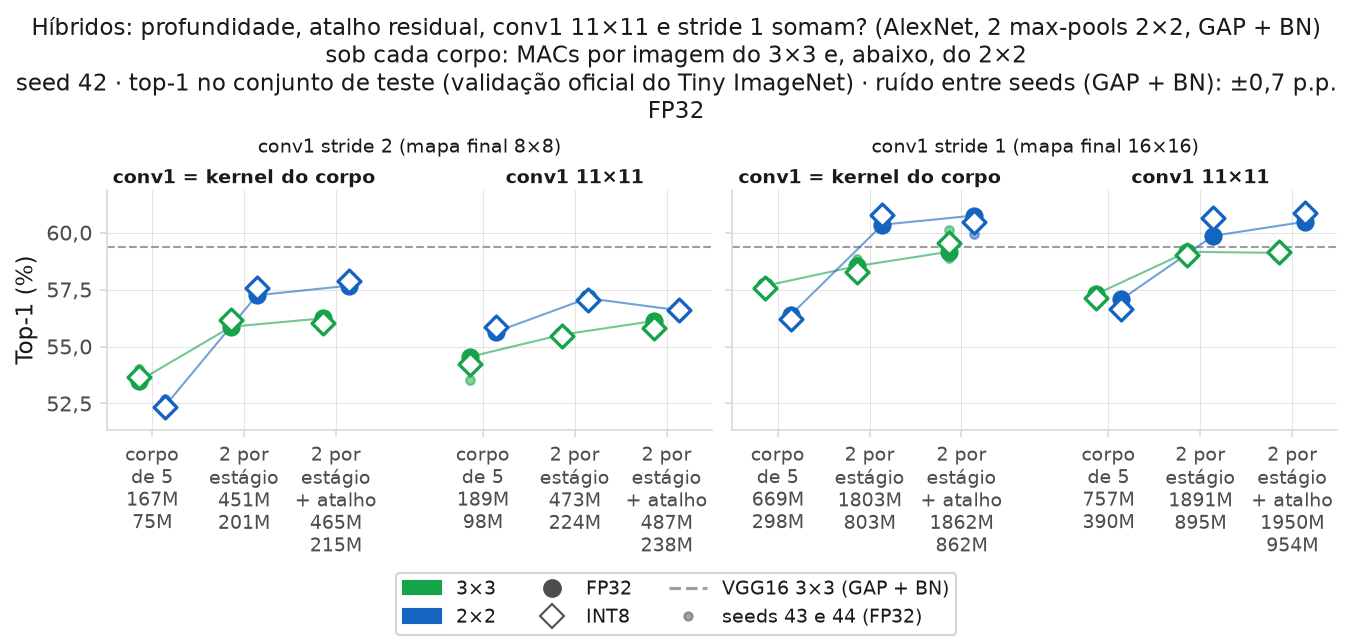
\includegraphics[width=\textwidth]{phase_13_hybrids/01_hybrids.png}
\caption{Todas as combinações (seed 42). Da esquerda para a direita, em cada grupo, o corpo fica mais profundo. O painel da direita (stride 1) fica acima do da esquerda
(stride 2), e o azul (2\by2) passa o verde (3\by3) quando há dois kernels por estágio. A linha tracejada é a VGG16 3\by3. Sob cada corpo estão os MACs do 3\by3 e do 2\by2.}
\label{fig:hibridos}
\end{figure*}

\begin{table}[!t]
\caption{Efeito de cada fator nas 24 combinações: mediana de B $-$ A (seed 42, p.p.)}
\label{tab:combinacoes}
\centering
\footnotesize
\setlength{\tabcolsep}{3pt}
\begin{tabular}{@{}lcccc@{}}
\toprule
\textbf{A $\rightarrow$ B} & \textbf{FP32} & \textbf{INT8} & \textbf{B acima} & \textbf{Faixa FP32} \\
\midrule
Stride da conv1: 2 $\rightarrow$ 1 & $+$3,03 & $+$3,40 & 12 de 12 & $+$1,43 a $+$4,16 \\
5 convs $\rightarrow$ 2 por estágio & $+$2,12 & $+$2,21 & 8 de 8 & $+$0,87 a $+$4,86 \\
Corpo 3\by3 $\rightarrow$ 2\by2 & $+$1,23 & $+$1,50 & 9 de 12 & $-$1,28 a $+$1,82 \\
2 por estágio $\rightarrow$ + atalho & $+$0,41 & $+$0,16 & 6 de 8 & $-$0,53 a $+$0,63 \\
Conv1 $\rightarrow$ 11\by11 & $-$0,12 & $-$0,19 & 4 de 12 & $-$1,08 a $+$3,25 \\
\bottomrule
\end{tabular}
\end{table}

O stride 1 é o maior fator e nunca falha, mas custa cerca de quatro vezes mais MACs. Dois kernels por estágio vêm em seguida e também nunca falham. O atalho residual fica dentro da
variação entre seeds, e seu sinal muda entre os pares. A conv1 11\by11 só ajuda no corpo de 5 convoluções (3 de 4 pares). Com dois kernels por estágio, sua mediana é de $-$0,20 p.p., ou seja,
a segunda convolução por estágio já entrega o que ela entregava.

O resultado mais curioso é o do kernel do corpo. Com 5 convoluções, a troca de 3\by3 por 2\by2 varia de $-$1,28 a $+$1,09 p.p. Com dois kernels por estágio, o 2\by2 vence nos 8 pares
(de $+$0,47 a $+$1,82 p.p., mediana de $+$1,4), com cerca de metade dos MACs.

Os dois maiores ganhos não se somam por inteiro. Partindo do 3\by3 com stride 2 (53,50\%), os ganhos separados de empilhar ($+$2,37) e de usar stride 1 ($+$4,16) levariam a 60,03\%. O
valor medido é 58,53\%. No 2\by2, a soma levaria a 61,24\% e o valor medido é 60,35\%. O corpo 2\by2 perde menos nessa combinação.

As melhores redes usam kernels 2\by2, dois por estágio, e stride 1. Com atalho, a rede chega a 60,75\% em FP32 e 60,46\% em INT8 (2,52M de parâmetros, 862M de MACs). Sem
atalho, chega a 60,35\% e 60,79\% (2,33M, 803M). A VGG16 3\by3 com GAP e BatchNorm fica em 59,35\% e 59,47\%, com 14,82M de parâmetros e 1255M de MACs (de 59,09\% a 59,37\% em 3 seeds). As
duas AlexNets ficam de 1,0 a 1,4 p.p. acima dela, com cerca de um sexto dos parâmetros e dois terços dos MACs. Como essas redes foram as melhores entre 24, a seed 42 pode estar favorecendo
as duas. Por isso, repetimos as duas com as seeds 43 e 44.
\pendente{Seeds 43 e 44 em andamento. Atualizar esta seção com a média das 3 seeds, a comparação do atalho por seed e a comparação com a VGG16 antes de tirar conclusões.}

\section{Discussão}

\subsection{Como desenhar uma rede para Winograd}

Os resultados apontam para algumas escolhas. Primeiro, acerte a geometria e o treino: stride baixo na conv1 para imagens pequenas, BatchNorm e GAP. Esses fatores pesam mais que o kernel. Segundo, não aumente
o kernel para ganhar acurácia: gastar a mais em largura ou em uma segunda convolução por estágio rende mais. Terceiro, evite redes em que a maior parte do cálculo fica em convoluções \textit{depthwise} ou 1\by1
se o alvo é Winograd. Quarto, não trate a quantização como obstáculo: o INT8 quase não muda a acurácia. O stride 1 é o fator mais caro: ele quadruplica os MACs, e cabe a cada projeto decidir se vale esse custo.

A escolha entre 2\by2 e 3\by3 depende do hardware. Em acurácia, com dois kernels por estágio, o 2\by2 vence e custa cerca de metade. Em um estudo paralelo do grupo com 14 redes em FPGA, porém, as transformações
testadas são do tipo F($m$,3), feitas para kernels 3\by3. O kernel 2\by2 fica fora delas. Nesse estudo, o tamanho da transformação é o que define o custo em acurácia: F(2,3) fica praticamente igual ao FP32 ($+$0,05 p.p.,
mediana), F(4,3) perde 5,1 p.p. e F(6,3) perde 18,9 p.p. Assim, um acelerador com F(2,3) e redes 3\by3 é hoje a opção sem custo medido. Usar 2\by2 exige um acelerador preparado para esse kernel.

\subsection{O que muda em relação ao trabalho anterior}

Sob a mesma receita, boa parte das diferenças entre redes de compensação desaparece. No relatório anterior \cite{souza2026relatorio}, um atalho residual em um bloco Fire \cite{iandola2016squeezenet} parecia ganhar mais de 6 p.p., mas os
treinos seguiam protocolos diferentes, inclusive no número de épocas. Agora, Fire fica em 54,57\% e FireBypass em 55,19\%, uma diferença de 0,62 p.p., dentro da variação. As redes Fire, FireBypass e as combinações com Fire e Bottleneck
ficam a menos de 1,5 p.p. umas das outras (de 54,40\% a 55,83\%, seed 42). O estudo de combinações aponta na mesma direção: o atalho não mostra ganho mensurável. Isso não invalida esses blocos, que continuam baratos, mas muda o motivo para usá-los.

As demais fases do projeto entram só como contexto, porque usaram protocolos diferentes. Medições anteriores em GPU indicaram que a aceleração Winograd depende de convoluções densas de stride 1. Em detecção, a compensação estrutural se transferiu só em
parte. Em atenção local, o tamanho da janela se comportou como o tamanho do kernel \cite{souza2026relatorio}.

\subsection{Limitações}

A maioria das comparações usa uma só seed. A receita é a mesma para todas as redes, mas não é a melhor para cada uma, e uma receita pode mudar a ordem entre arquiteturas \cite{bello2021revisiting,wightman2021resnet}. Os dados são de baixa
resolução: 64 px e 32 px, e as imagens de 224 px são apenas ampliações. A parcela de MACs mede só a geometria das camadas, e não medimos a vazão em um acelerador real. Não comparamos latência entre redes, porque os treinos rodaram em máquinas diferentes
(RTX 4090, RTX 4060 Ti e GTX 1080 Ti). Essa diferença de máquina faz parte da variação entre execuções e também afeta a seed 42 do estudo de combinações: as duas melhores redes foram treinadas em GPUs diferentes.

\section{Conclusão}

Restringir o kernel custa pouco. Trocar os kernels originais da AlexNet por 3\by3 custa cerca de 1,5 p.p., e com GAP e BatchNorm nem isso. O 2\by2 custa mais, porém esse custo vem de fazer menos cálculo: com os mesmos MACs, ele empata com o 3\by3. A geometria da
rede, o BatchNorm, o Dropout e o pré-treino pesam mais, e a quantização INT8 quase não pesa. Duas convoluções pequenas por estágio recuperam a perda, e com elas o 2\by2 passa a vencer o 3\by3 pela metade do custo. Essas conclusões se repetem com outras taxas de aprendizado e no CIFAR-100.
Para quem projeta redes para aceleradores Winograd, a mensagem é simples: não é preciso manter kernels grandes no corpo da rede para ter boa acurácia.

\section{Trabalhos Futuros}

O passo seguinte é concluir as seeds 43 e 44 das melhores redes. Depois, queremos reavaliar todas as redes no mesmo tipo de máquina, para comparar latência; medir a vazão em um acelerador real; testar blocos Bottleneck e Fire sobre o melhor corpo, para ver se reduzem o custo sem perder
acurácia; investigar a perda da MobileNetV2 pré-treinada em INT8; e repetir as comparações principais em imagens de resolução maior.

\section*{Agradecimentos}
Experimentos utilizaram recursos da infraestrutura PCAD (http://pcad.inf.ufrgs.br).

\renewcommand{\refname}{Referências}
\begin{thebibliography}{00}

\bibitem{lavin2016fast}
A. Lavin and S. Gray, ``Fast algorithms for convolutional neural networks,'' in \textit{Proc. IEEE Conf. Computer Vision and Pattern Recognition (CVPR)}, 2016.

\bibitem{barabasz2020error}
B. Barabasz, A. Anderson, K. M. Soodhalter, and D. Gregg, ``Error analysis and improving the accuracy of Winograd convolution for deep neural networks,'' \textit{ACM Transactions on Mathematical Software}, vol. 46, no. 4, Art. 37, 2020.

\bibitem{krizhevsky2012imagenet}
A. Krizhevsky, I. Sutskever, and G. E. Hinton, ``ImageNet classification with deep convolutional neural networks,'' in \textit{Advances in Neural Information Processing Systems (NeurIPS)}, 2012.

\bibitem{simonyan2015very}
K. Simonyan and A. Zisserman, ``Very deep convolutional networks for large-scale image recognition,'' in \textit{International Conference on Learning Representations (ICLR)}, 2015.

\bibitem{liu2022convnext}
Z. Liu, H. Mao, C.-Y. Wu, C. Feichtenhofer, T. Darrell, and S. Xie, ``A ConvNet for the 2020s,'' in \textit{Proc. IEEE/CVF Conf. Computer Vision and Pattern Recognition (CVPR)}, 2022.

\bibitem{ding2022scaling}
X. Ding, X. Zhang, Y. Zhou, J. Han, G. Ding, and J. Sun, ``Scaling up your kernels to 31x31: Revisiting large kernel design in CNNs,'' in \textit{Proc. IEEE/CVF Conf. Computer Vision and Pattern Recognition (CVPR)}, 2022.

\bibitem{souza2026relatorio}
R. S. de Souza and M. G. da Silva, ``Restrição do tamanho de kernel em CNNs para aceleração Winograd,'' relatório de pesquisa, Instituto de Informática, UFRGS, 2026.

\bibitem{bello2021revisiting}
I. Bello \textit{et al.}, ``Revisiting ResNets: Improved training and scaling strategies,'' in \textit{Advances in Neural Information Processing Systems (NeurIPS)}, 2021.

\bibitem{wightman2021resnet}
R. Wightman, H. Touvron, and H. Jégou, ``ResNet strikes back: An improved training procedure in timm,'' \textit{arXiv preprint arXiv:2110.00476}, 2021.

\bibitem{radosavovic2019network}
I. Radosavovic, J. Johnson, S. Xie, W.-Y. Lo, and P. Dollár, ``On network design spaces for visual recognition,'' in \textit{Proc. IEEE/CVF International Conference on Computer Vision (ICCV)}, 2019.

\bibitem{le2015tiny}
Y. Le and X. Yang, ``Tiny ImageNet visual recognition challenge,'' Stanford CS231N Report, 2015.

\bibitem{cawley2010overfitting}
G. C. Cawley and N. L. C. Talbot, ``On over-fitting in model selection and subsequent selection bias in performance evaluation,'' \textit{Journal of Machine Learning Research}, vol. 11, 2010.

\bibitem{krizhevsky2009learning}
A. Krizhevsky, ``Learning multiple layers of features from tiny images,'' Technical Report, University of Toronto, 2009.

\bibitem{he2019bag}
T. He, Z. Zhang, H. Zhang, Z. Zhang, J. Xie, and M. Li, ``Bag of tricks for image classification with convolutional neural networks,'' in \textit{Proc. IEEE/CVF Conf. Computer Vision and Pattern Recognition (CVPR)}, 2019.

\bibitem{szegedy2016rethinking}
C. Szegedy, V. Vanhoucke, S. Ioffe, J. Shlens, and Z. Wojna, ``Rethinking the Inception architecture for computer vision,'' in \textit{Proc. IEEE Conf. Computer Vision and Pattern Recognition (CVPR)}, 2016.

\bibitem{chrabaszcz2017downsampled}
P. Chrabaszcz, I. Loshchilov, and F. Hutter, ``A downsampled variant of ImageNet as an alternative to the CIFAR datasets,'' \textit{arXiv preprint arXiv:1707.08819}, 2017.

\bibitem{cubuk2019autoaugment}
E. D. Cubuk, B. Zoph, D. Mané, V. Vasudevan, and Q. V. Le, ``AutoAugment: Learning augmentation strategies from data,'' in \textit{Proc. IEEE Conf. Computer Vision and Pattern Recognition (CVPR)}, 2019, pp. 113--123.

\bibitem{he2015delving}
K. He, X. Zhang, S. Ren, and J. Sun, ``Delving deep into rectifiers: Surpassing human-level performance on ImageNet classification,'' in \textit{Proc. IEEE International Conference on Computer Vision (ICCV)}, 2015.

\bibitem{he2016deep}
K. He, X. Zhang, S. Ren, and J. Sun, ``Deep residual learning for image recognition,'' in \textit{Proc. IEEE Conf. Computer Vision and Pattern Recognition (CVPR)}, 2016.

\bibitem{wu2019convolution}
S. Wu, G. Wang, P. Tang, F. Chen, and L. Shi, ``Convolution with even-sized kernels and symmetric padding,'' in \textit{Advances in Neural Information Processing Systems (NeurIPS)}, 2019.

\bibitem{jacob2018quantization}
B. Jacob \textit{et al.}, ``Quantization and training of neural networks for efficient integer-arithmetic-only inference,'' in \textit{Proc. IEEE Conf. Computer Vision and Pattern Recognition (CVPR)}, 2018.

\bibitem{wu2020integer}
H. Wu, P. Judd, X. Zhang, M. Isaev, and P. Micikevicius, ``Integer quantization for deep learning inference: Principles and empirical evaluation,'' \textit{arXiv preprint arXiv:2004.09602}, 2020.

\bibitem{nagel2021white}
M. Nagel, M. Fournarakis, R. A. Amjad, Y. Bondarenko, M. van Baalen, and T. Blankevoort, ``A white paper on neural network quantization,'' \textit{arXiv preprint arXiv:2106.08295}, 2021.

\bibitem{bouthillier2021accounting}
X. Bouthillier \textit{et al.}, ``Accounting for variance in machine learning benchmarks,'' in \textit{Proc. Machine Learning and Systems (MLSys)}, 2021.

\bibitem{luo2016understanding}
W. Luo, Y. Li, R. Urtasun, and R. Zemel, ``Understanding the effective receptive field in deep convolutional neural networks,'' in \textit{Advances in Neural Information Processing Systems (NeurIPS)}, 2016.

\bibitem{hooker2019what}
S. Hooker, A. Courville, G. Clark, Y. Dauphin, and A. Frome, ``What do compressed deep neural networks forget?'' \textit{arXiv preprint arXiv:1911.05248}, 2019.

\bibitem{kendall1938new}
M. G. Kendall, ``A new measure of rank correlation,'' \textit{Biometrika}, vol. 30, no. 1--2, pp. 81--93, 1938.

\bibitem{li2020rethinking}
H. Li \textit{et al.}, ``Rethinking the hyperparameters for fine-tuning,'' in \textit{International Conference on Learning Representations (ICLR)}, 2020.

\bibitem{iandola2016squeezenet}
F. N. Iandola, S. Han, M. W. Moskewicz, K. Ashraf, W. J. Dally, and K. Keutzer, ``SqueezeNet: AlexNet-level accuracy with 50x fewer parameters and $<$0.5MB model size,'' \textit{arXiv preprint arXiv:1602.07360}, 2016.

\end{thebibliography}

\appendix
\subsection{Figuras de apoio}
\label{sec:apendice}

As figuras a seguir trazem o detalhe por trás do texto: as curvas de treino, que mostram que as redes param de melhorar antes do fim das épocas, e as barras de cada fator da Tabela~\ref{tab:fatores_efeito}.

\begin{figure*}[!t]
\centering
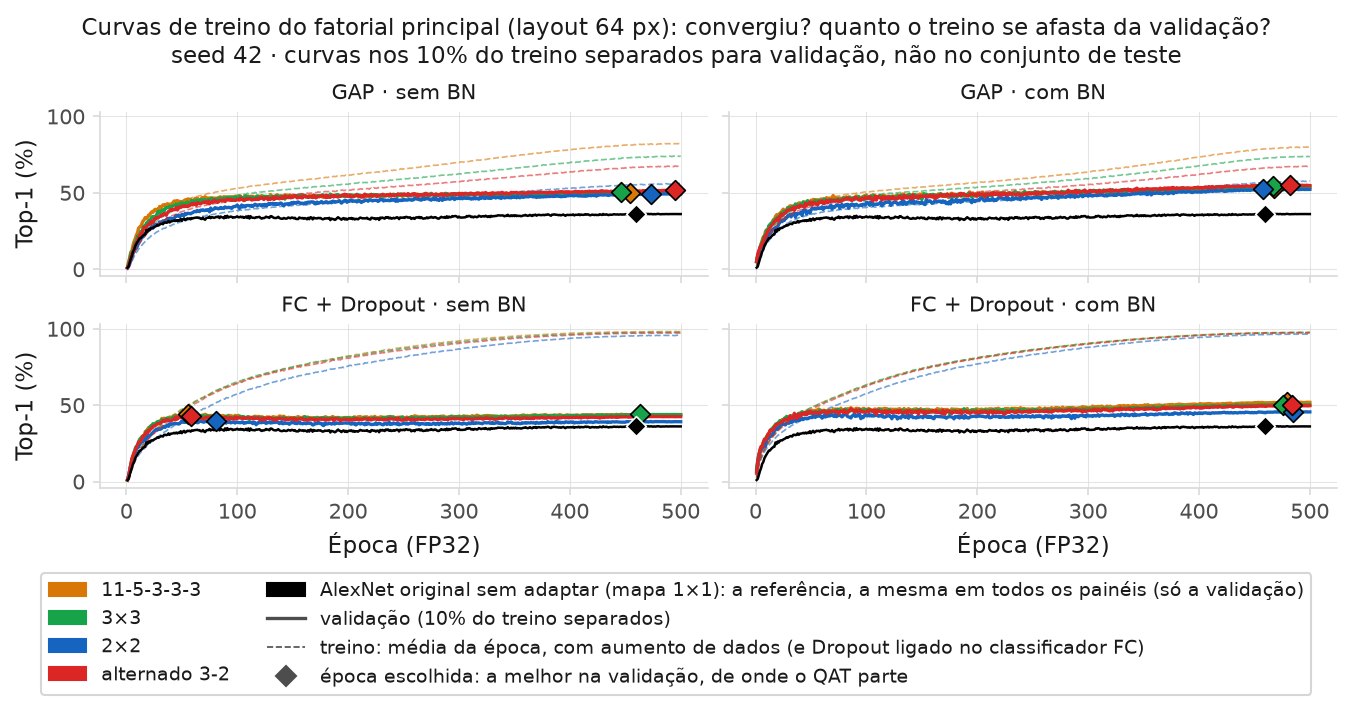
\includegraphics[width=0.74\textwidth,trim=0 0 0 38.4,clip]{phase_11_kernel_size_comparison/18_training_curves.png}
\caption{Curvas de treino em FP32 (AlexNet de layout 64 px, seed 42), medidas nos 10\% do treino separados para validação. As redes com FC chegam perto de 100\% no treino, enquanto a validação fica parada. Nas redes com FC sem BatchNorm, a melhor época costuma vir cedo: são os casos marcados no texto.}
\label{fig:curvas_fp32}
\end{figure*}

\begin{figure*}[!t]
\centering
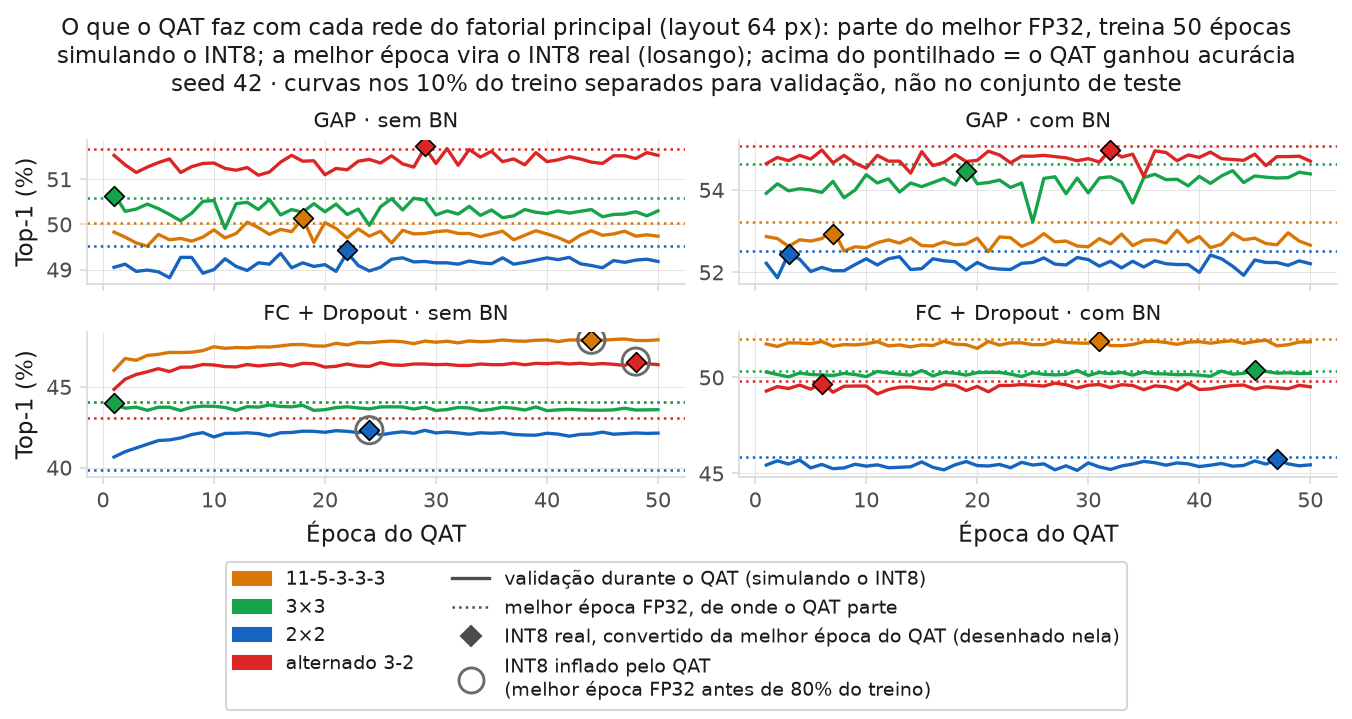
\includegraphics[width=0.74\textwidth,trim=0 0 0 52.3,clip]{phase_11_kernel_size_comparison/19_qat_curves.png}
\caption{Curvas do QAT nas mesmas redes. O pontilhado é o FP32 de onde o QAT parte, e o losango é a época convertida para INT8. Só as redes com anel sobem claramente acima do ponto de partida: é o treino extra descrito na Seção~\ref{sec:int8}.}
\label{fig:curvas_qat}
\end{figure*}

\begin{figure*}[!t]
\centering
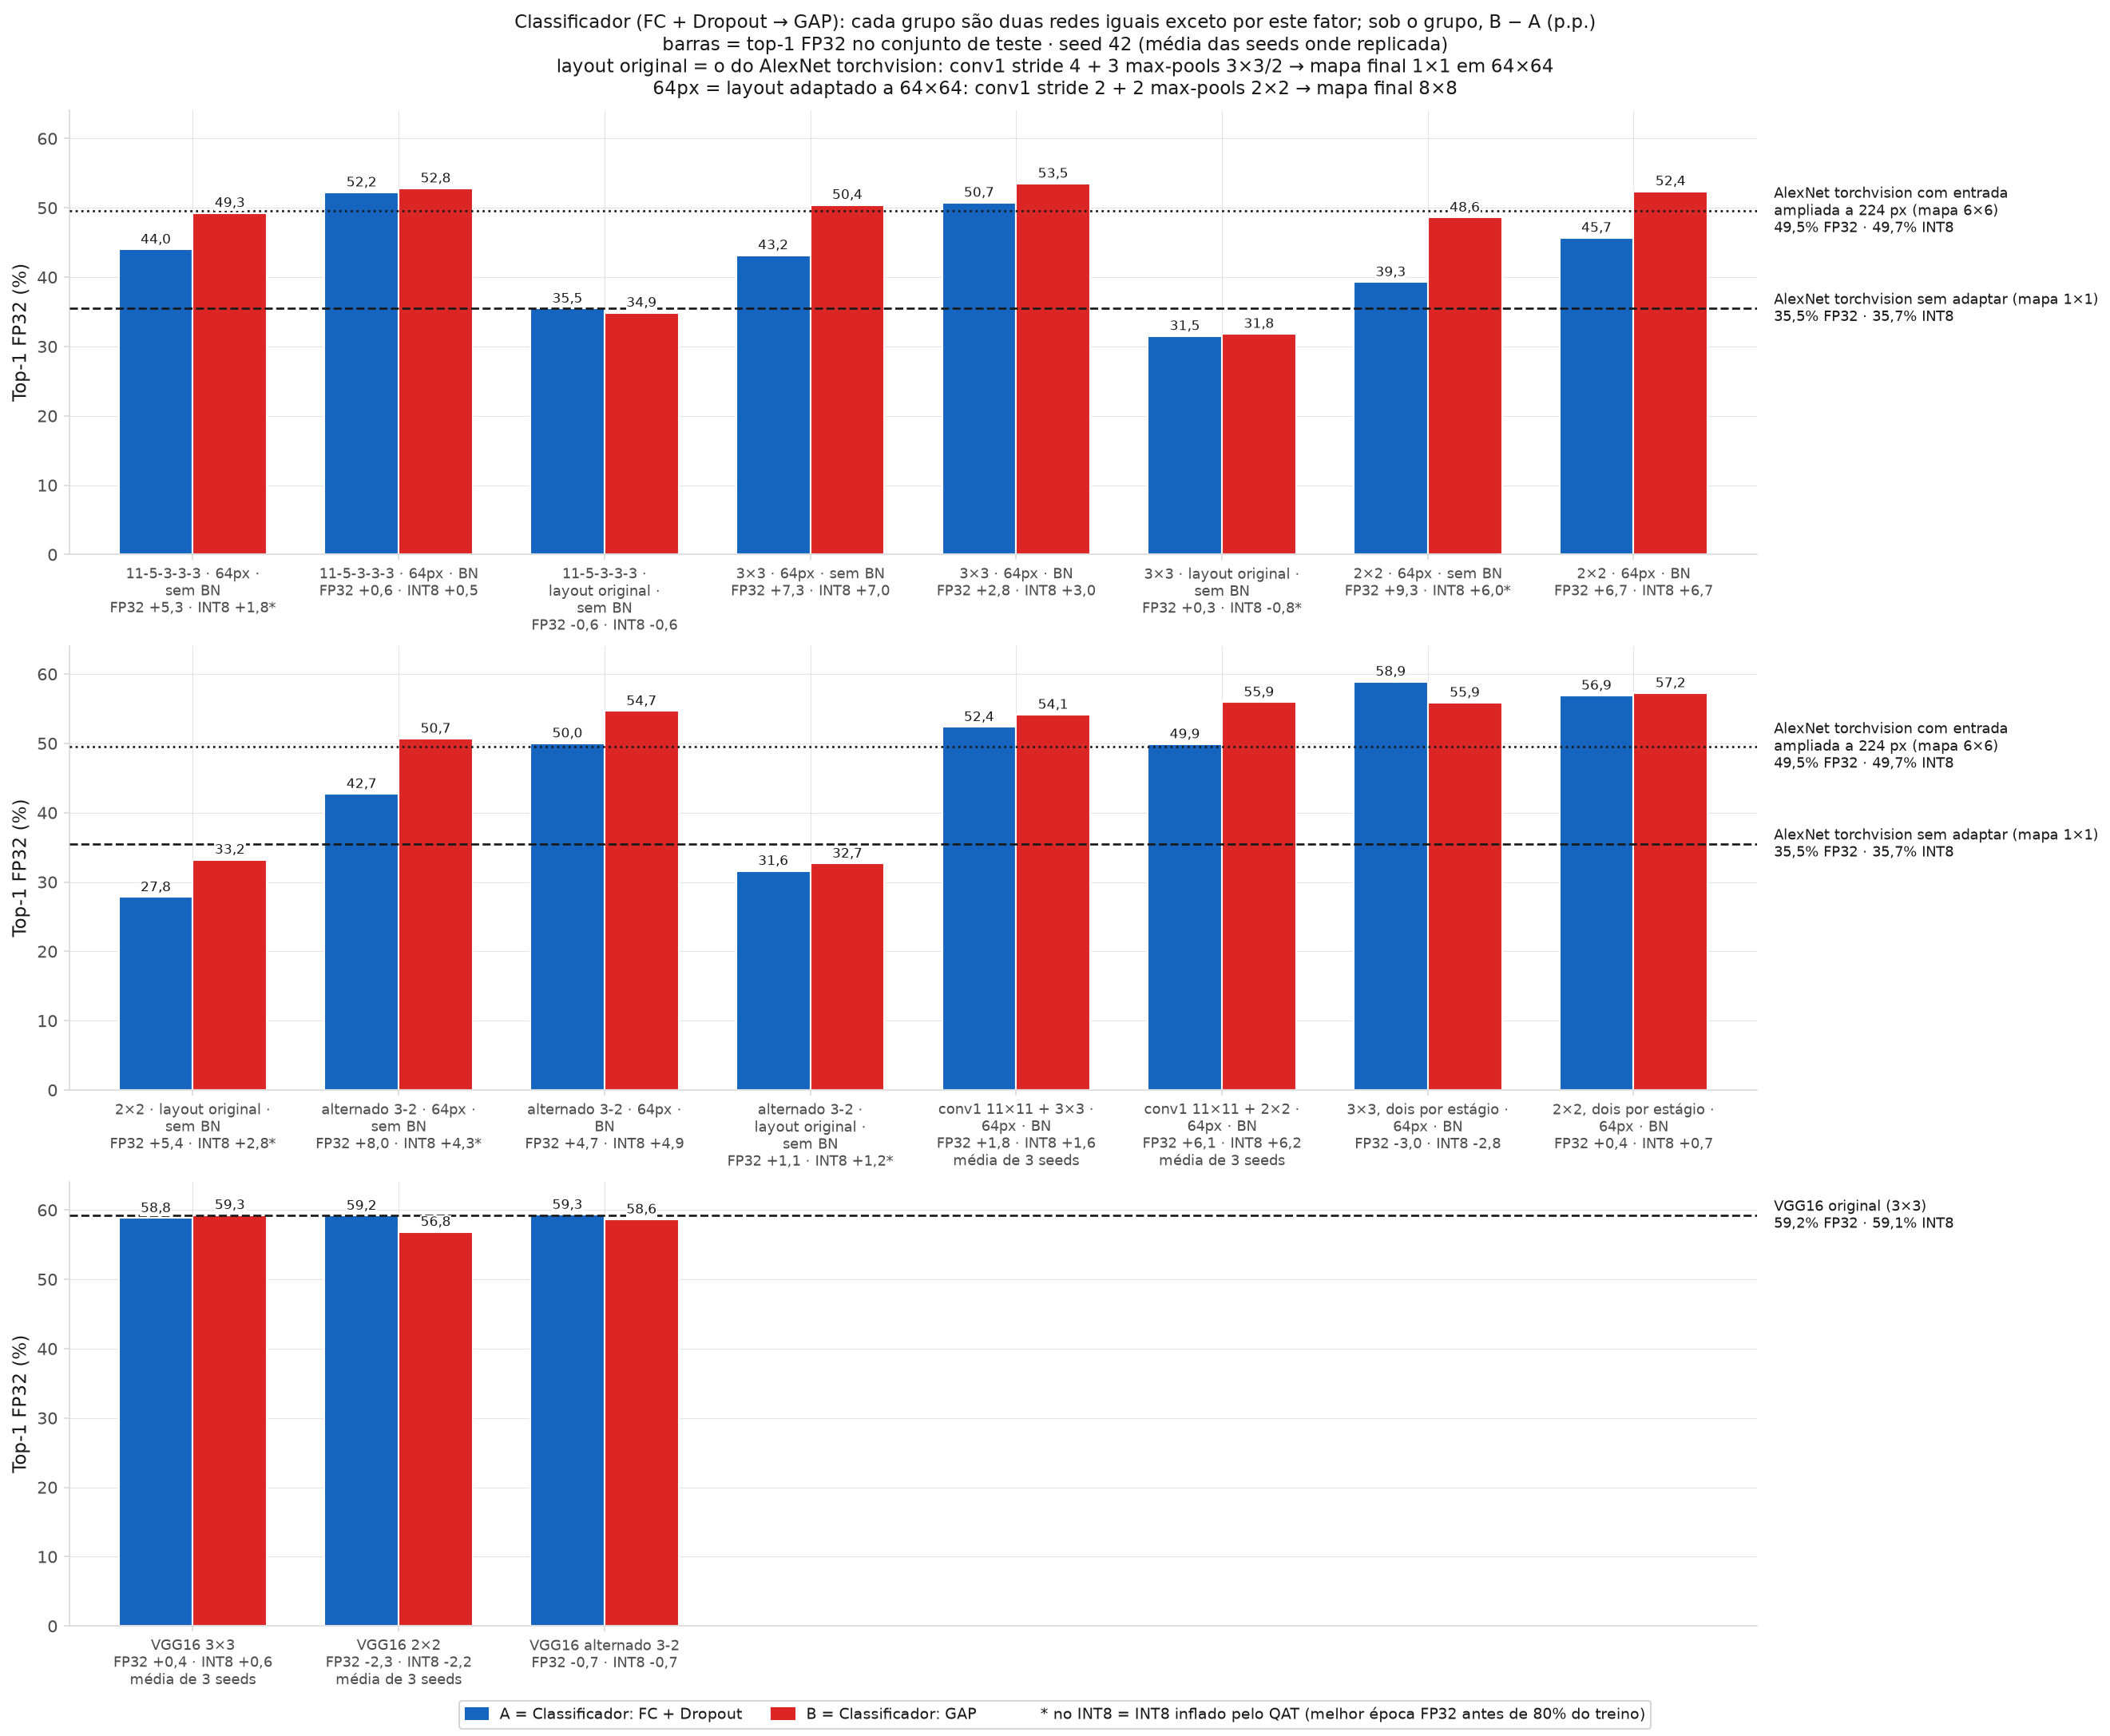
\includegraphics[width=0.72\textwidth]{phase_11_kernel_size_comparison/04_head_fc_vs_gap.png}
\caption{Classificador: FC + Dropout contra GAP, em pares de redes iguais no resto.}
\label{fig:cabeca}
\end{figure*}

\begin{figure*}[!t]
\centering
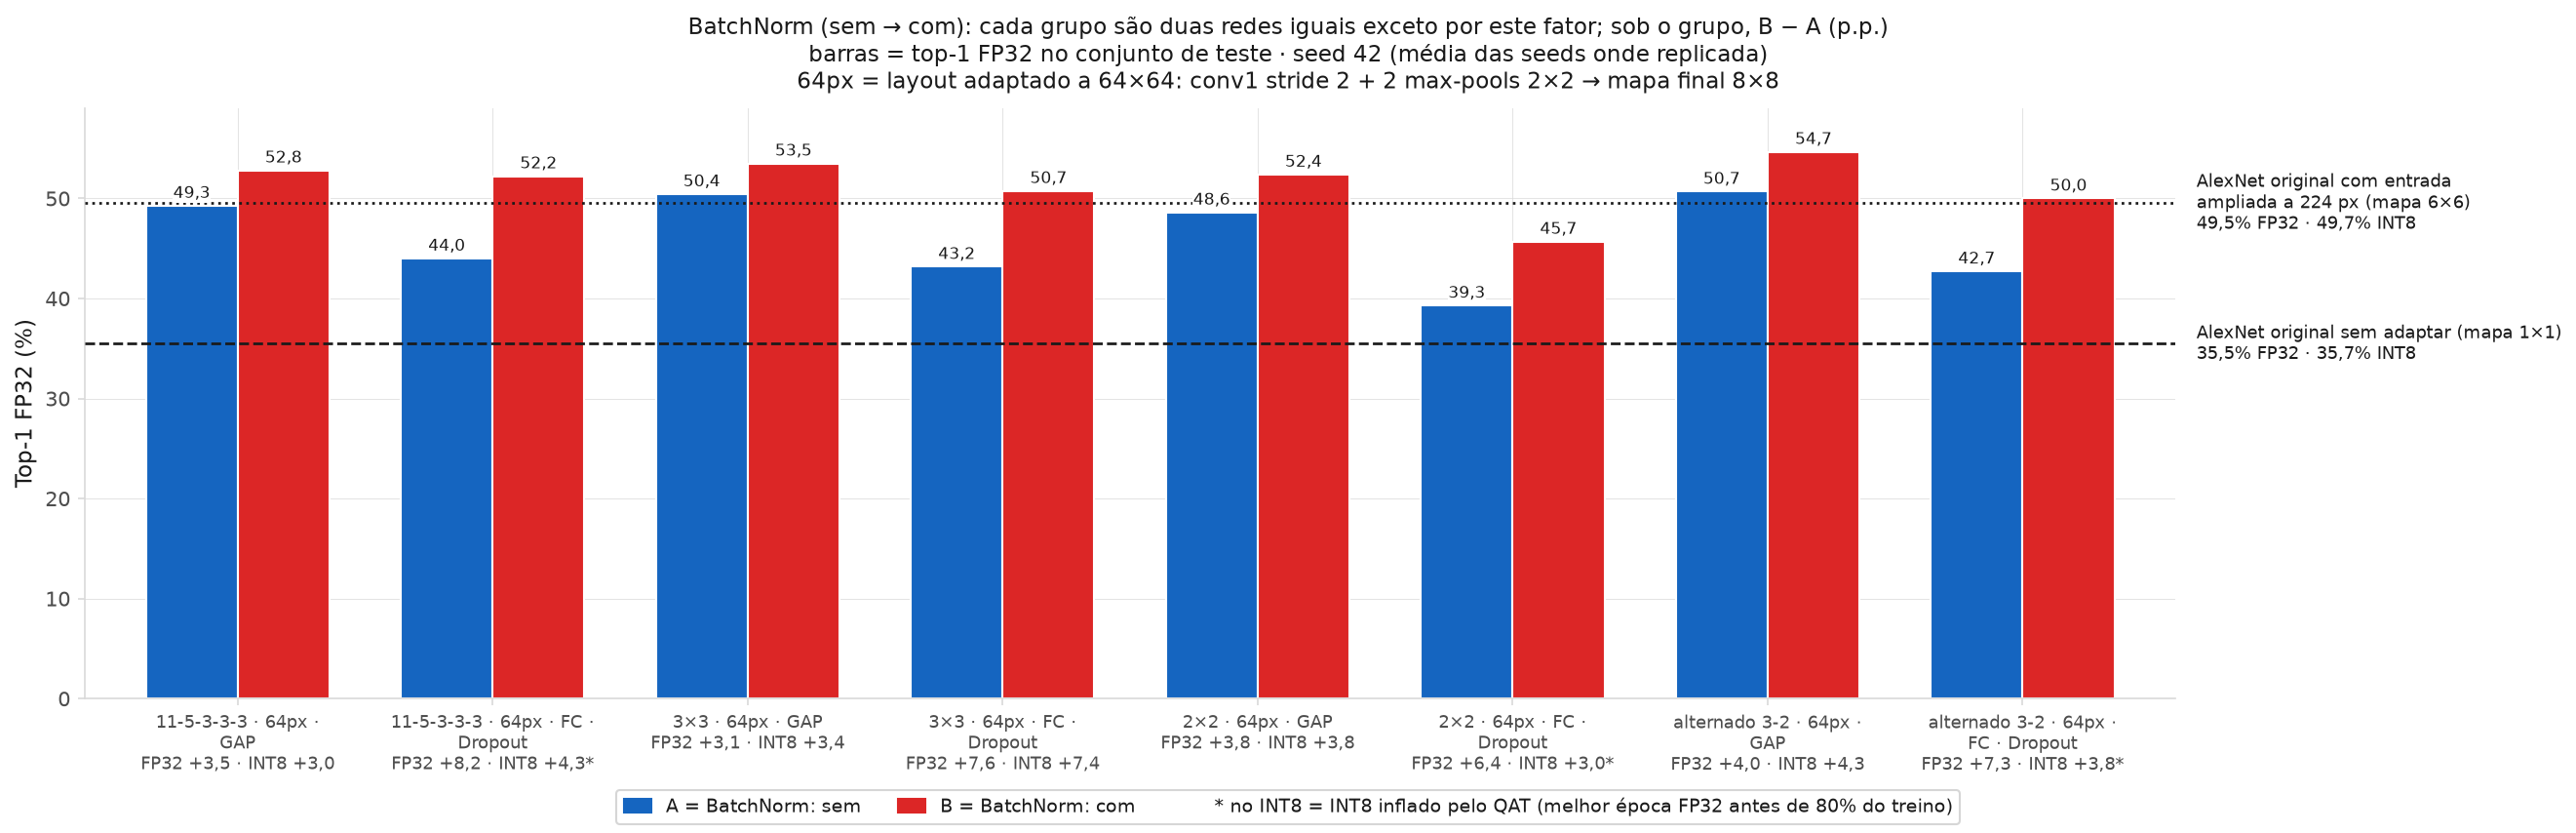
\includegraphics[width=\textwidth]{phase_11_kernel_size_comparison/09_batchnorm.png}
\caption{BatchNorm: sem contra com, em pares de redes iguais no resto. O BatchNorm ganha em todos os pares.}
\label{fig:bn}
\end{figure*}

\begin{figure*}[!t]
\centering
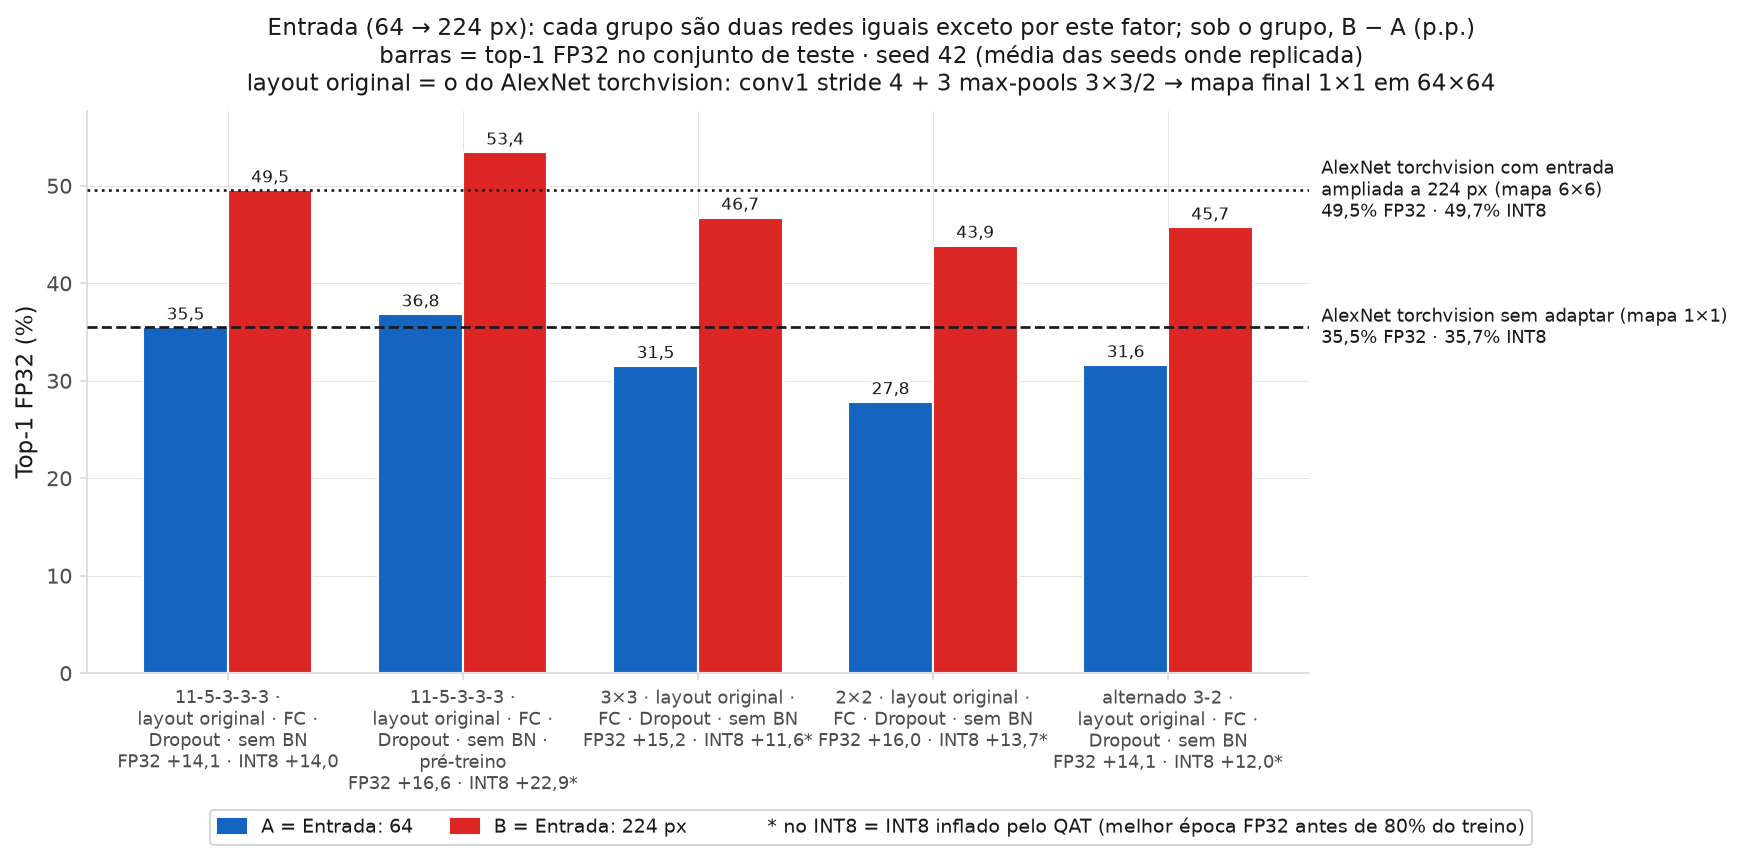
\includegraphics[width=0.6\textwidth]{phase_11_kernel_size_comparison/23_input_224.png}
\caption{Entrada de 64 px contra a mesma imagem ampliada para 224 px, com o layout original.}
\label{fig:entrada}
\end{figure*}

\begin{figure*}[!t]
\centering
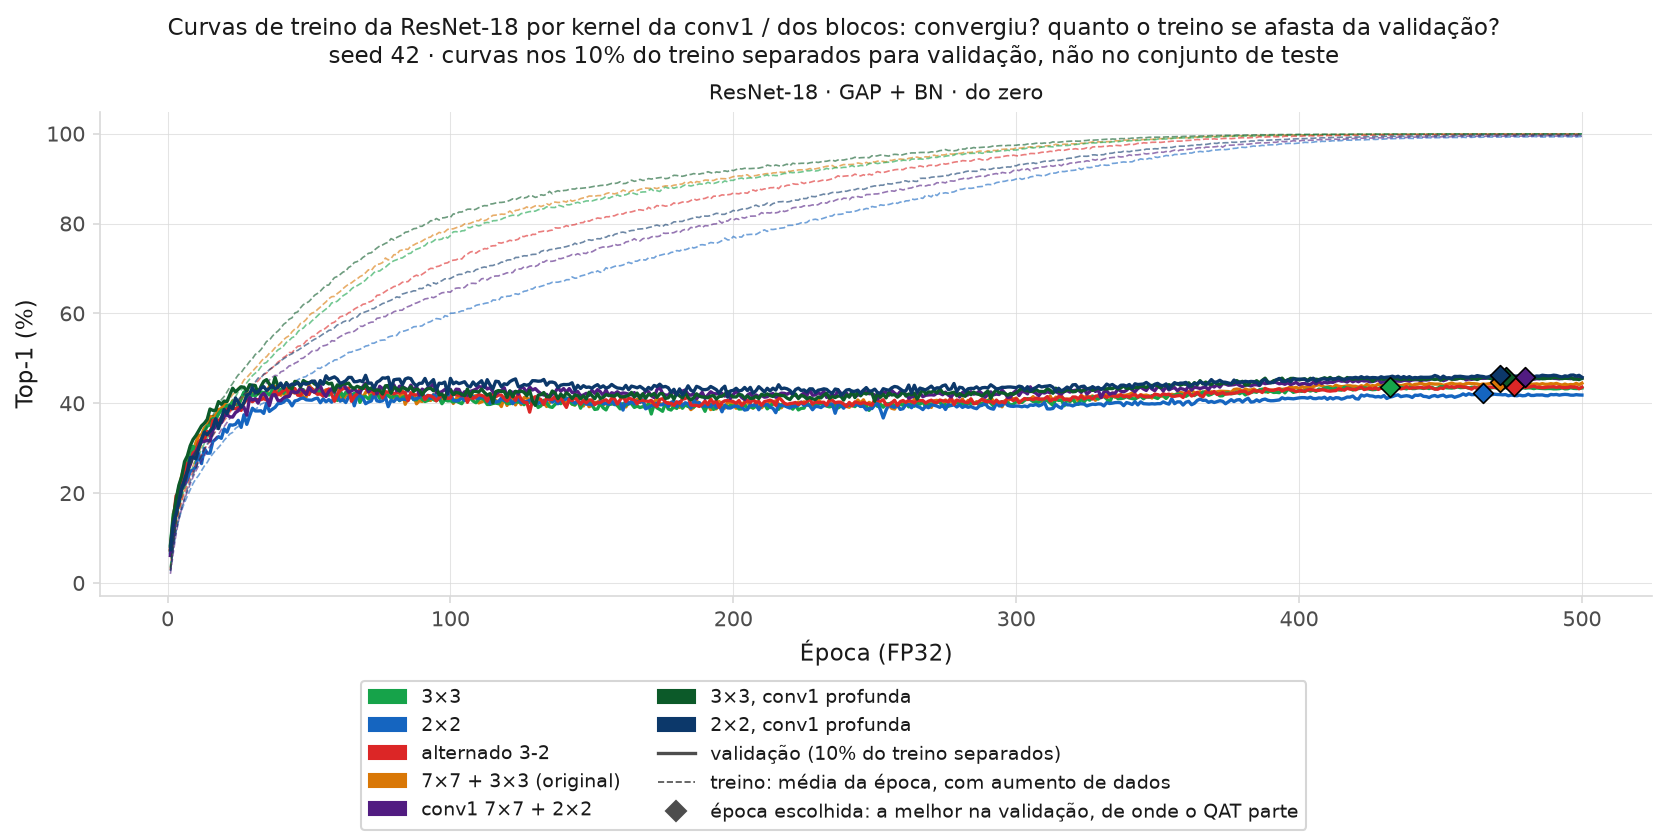
\includegraphics[width=0.6\textwidth]{phase_11_kernel_size_comparison/29_resnet_training_curves.png}
\caption{Curvas de treino da ResNet-18, por kernel da primeira camada e dos blocos (seed 42). O treino chega perto de 100\%, enquanto a validação fica entre 40\% e 46\%.}
\label{fig:curvas_resnet}
\end{figure*}

\begin{figure*}[!t]
\centering
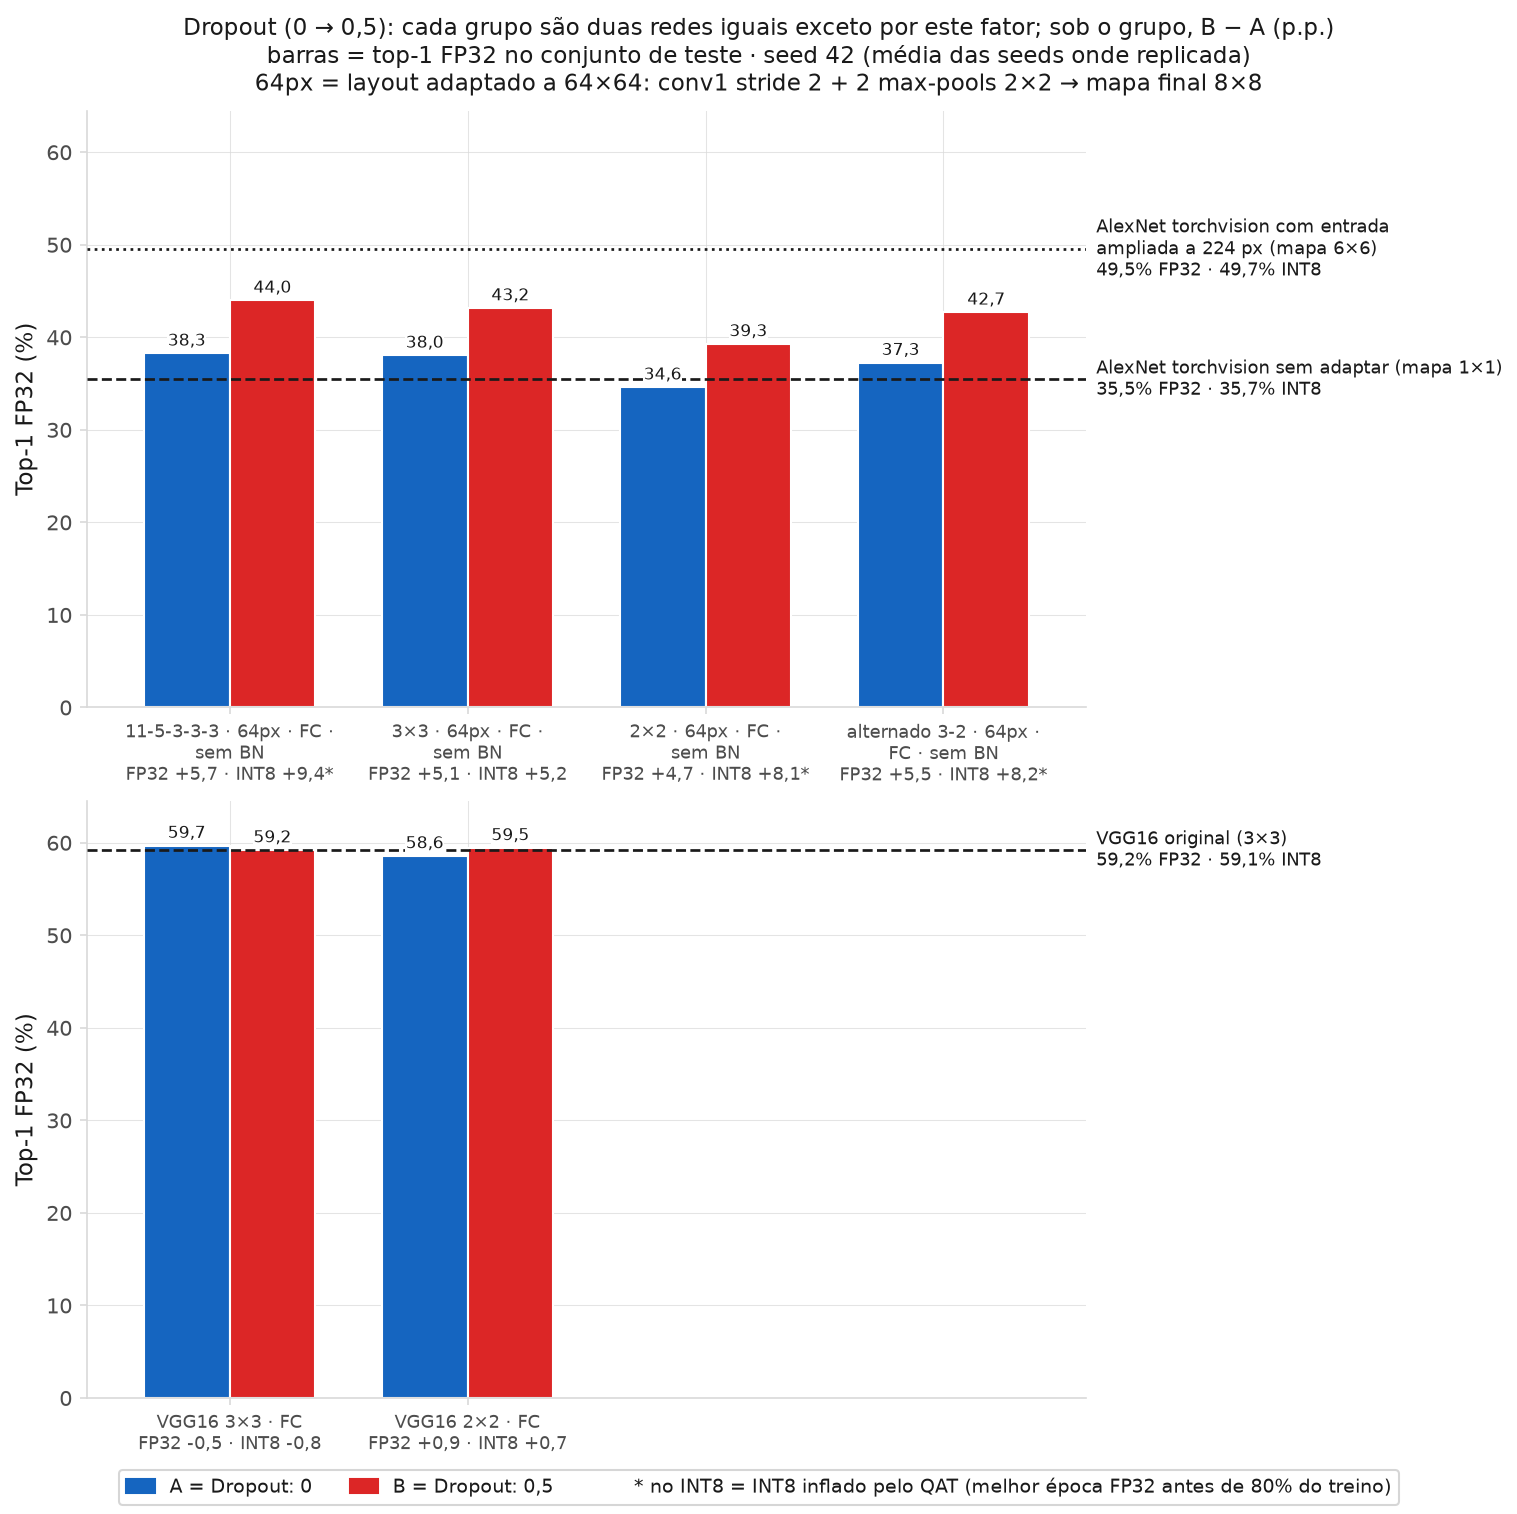
\includegraphics[width=0.5\textwidth]{phase_11_kernel_size_comparison/07_dropout.png}\hfill
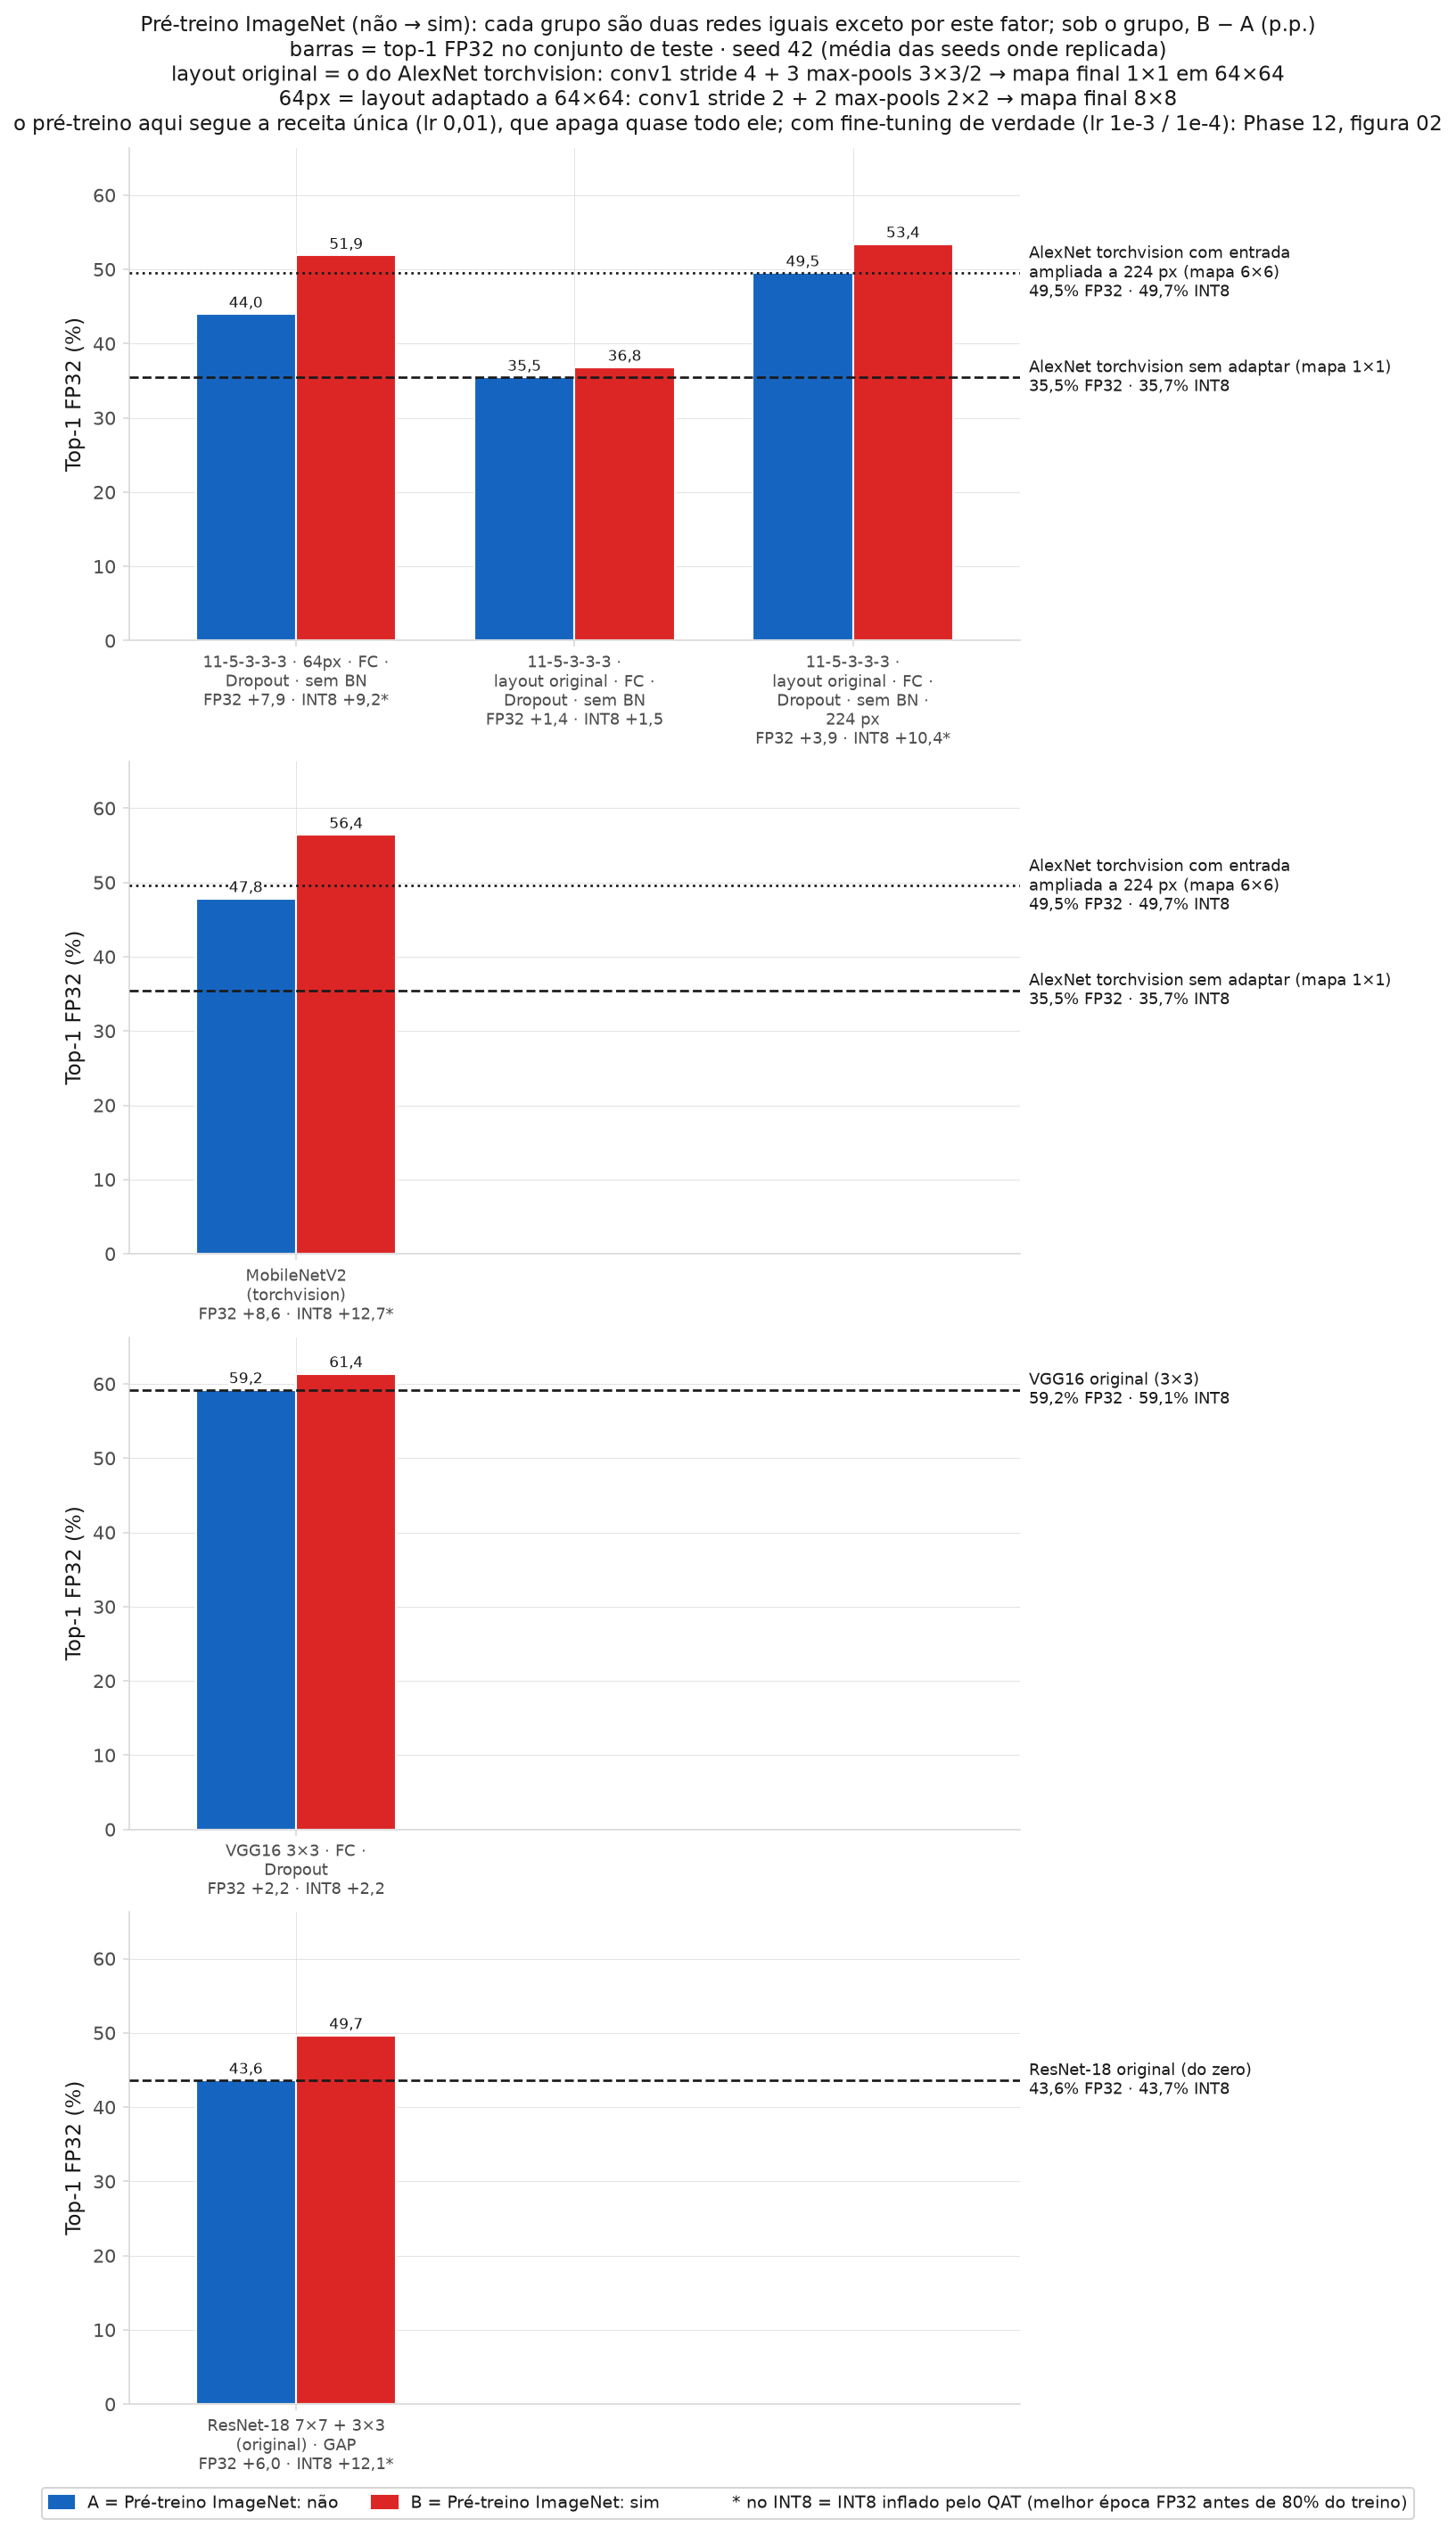
\includegraphics[width=0.48\textwidth]{phase_11_kernel_size_comparison/08_pretraining.png}
\caption{À esquerda, Dropout de 0 a 0,5, só no classificador FC. À direita, pré-treino na ImageNet com a receita única (taxa de aprendizado 0,01).}
\label{fig:dropout_pretreino}
\end{figure*}

\end{document}
